\subsubsection{Teacher Use Cases}

The Teacher actor is centered on pedagogical production and publication
workflows. The most relevant use cases are training path creation, content
maintenance, quiz publication, and submission for approval.

\dotsection{\textbf{Specification of the Use Case View Analytics \& Performance}}
\begin{table}[H]
    \centering
    \caption{Use Case Specification: View Analytics \& Performance}
    \begin{tabular}{|p{3.5cm}|p{10.5cm}|}
        \hline
        \textbf{Title}          & View Analytics \& Performance                                                                                   \\
        \hline
        \textbf{Summary}        & Teacher reviews enrollment statistics, completion rates, and learner performance for their training paths \\
        \hline
        \textbf{Actor}          & Teacher                                                                                                   \\
        \hline
        \textbf{Precondition}   & The teacher is authenticated and has at least one published training path                                 \\
        \hline
        \textbf{Post-condition} & The teacher views analytics data for their training paths                                                 \\
        \hline
        \textbf{Basic Scenario} & \begin{minipage}[t]{\linewidth}
                                      \begin{enumerate}[topsep=0pt,itemsep=1pt,parsep=0pt,partopsep=0pt]
                                          \item Teacher opens the teaching analytics dashboard
                                          \item System retrieves enrollment counts, completion rates, and average quiz scores
                                                per training path
                                          \item System displays charts and tables with time-series trends
                                          \item Teacher may filter analytics by date range or training path
                                          \item Teacher may drill down into individual module or unit performance
                                      \end{enumerate}
                                  \end{minipage}                \\
        \hline
        \textbf{Error Scenario} & \begin{minipage}[t]{\linewidth}
                                      \begin{enumerate}[topsep=0pt,itemsep=1pt,parsep=0pt,partopsep=0pt]
                                          \item If no training paths exist, the system displays an empty-state message
                                          \item If analytics data is still computing, the system shows a loading indicator
                                      \end{enumerate}
                                  \end{minipage}                   \\
        \hline
    \end{tabular}
    \label{tab:teacher-analytics}
\end{table}

\iffalse
\subsubsubsection[View Analytics \& Performance]{Refinement of the Use Case View Analytics \& Performance} Figure
\ref{fig:teacher-view-analytics-and-performance-use-case} presents the refinement of the
Use Case View Analytics \& Performance for the Teacher actor. This use case includes
the following sub-use cases:
\begin{figure}[H]
    \centering
    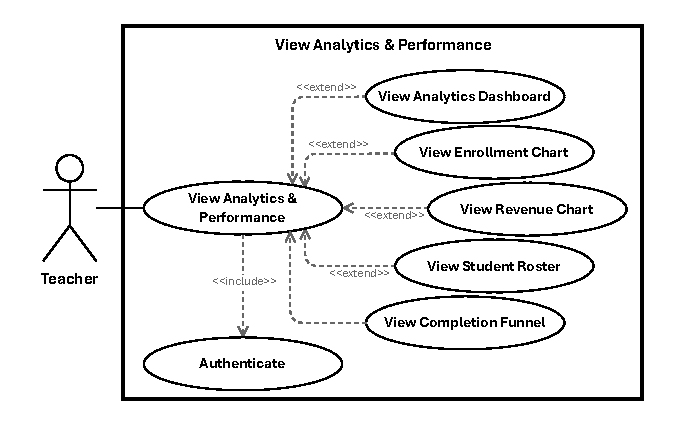
\includegraphics[width=\textwidth]{assets/chapter3/teacher-view-analytics-and-performance-use-case}
    \caption{Use Case View Analytics \& Performance}
    \label{fig:teacher-view-analytics-and-performance-use-case}
\end{figure}
\dotsection{\textbf{Specification of the Use Case View Analytics Dashboard}}
\begin{table}[H]
    \centering
    \caption{Use Case Specification: View Analytics Dashboard}
    \begin{tabular}{|p{3.5cm}|p{10.5cm}|}
        \hline
        \textbf{Title}          & View Analytics Dashboard                                                                 \\
        \hline
        \textbf{Summary}        & Teacher views comprehensive analytics dashboard with KPIs, charts, and trends \\
        \hline
        \textbf{Actor}          & Teacher                                                                      \\
        \hline
        \textbf{Precondition}   & Teacher is authenticated and has at least one published training path        \\
        \hline
        \textbf{Post-condition} & Teacher views analytics data for all training paths with visualizations      \\
        \hline
        \textbf{Basic Scenario} & \begin{minipage}[t]{\linewidth}
                                      \begin{enumerate}[topsep=0pt,itemsep=1pt,parsep=0pt,partopsep=0pt]
                                          \item Teacher navigates to analytics dashboard
                                          \item System retrieves key performance indicators
                                          \item System displays KPI cards with totals and averages
                                          \item System shows enrollment and revenue charts
                                          \item System displays top performing training paths
                                          \item Teacher may filter by time period
                                      \end{enumerate}
                                  \end{minipage} \\
        \hline
        \textbf{Error Scenario} & \begin{minipage}[t]{\linewidth}
                                      \begin{enumerate}[topsep=0pt,itemsep=1pt,parsep=0pt,partopsep=0pt]
                                          \item If no training paths exist, system displays empty state
                                          \item If analytics service unavailable, system shows cached data with warning
                                      \end{enumerate}
                                  \end{minipage} \\
        \hline
    \end{tabular}
    \label{tab:teacher-analytics-dashboard}
\end{table}
\dotsection{\textbf{Specification of the Use Case View Enrollment Chart}}
\begin{table}[H]
    \centering
    \caption{Use Case Specification: View Enrollment Chart}
    \begin{tabular}{|p{3.5cm}|p{10.5cm}|}
        \hline
        \textbf{Title}          & View Enrollment Chart                                                                 \\
        \hline
        \textbf{Summary}        & Teacher views enrollment trends over time with visual chart representation    \\
        \hline
        \textbf{Actor}          & Teacher                                                                      \\
        \hline
        \textbf{Precondition}   & Teacher is authenticated and has training paths with enrollment data          \\
        \hline
        \textbf{Post-condition} & Teacher views enrollment chart with time-series data and trends              \\
        \hline
        \textbf{Basic Scenario} & \begin{minipage}[t]{\linewidth}
                                      \begin{enumerate}[topsep=0pt,itemsep=1pt,parsep=0pt,partopsep=0pt]
                                          \item Teacher opens analytics dashboard
                                          \item Teacher navigates to enrollment chart section
                                          \item System retrieves enrollment data by date
                                          \item System displays line or bar chart with enrollment trends
                                          \item Teacher may filter by time period (7d, 30d, 90d, 1y)
                                          \item System updates chart with selected period
                                      \end{enumerate}
                                  \end{minipage} \\
        \hline
        \textbf{Error Scenario} & \begin{minipage}[t]{\linewidth}
                                      \begin{enumerate}[topsep=0pt,itemsep=1pt,parsep=0pt,partopsep=0pt]
                                          \item If no enrollment data exists, system displays empty chart
                                          \item If chart generation fails, system displays error message
                                      \end{enumerate}
                                  \end{minipage} \\
        \hline
    \end{tabular}
    \label{tab:teacher-enrollment-chart}
\end{table}
\dotsection{\textbf{Specification of the Use Case View Revenue Chart}}
\begin{table}[H]
    \centering
    \caption{Use Case Specification: View Revenue Chart}
    \begin{tabular}{|p{3.5cm}|p{10.5cm}|}
        \hline
        \textbf{Title}          & View Revenue Chart                                                                 \\
        \hline
        \textbf{Summary}        & Teacher views revenue trends over time with visual chart representation      \\
        \hline
        \textbf{Actor}          & Teacher                                                                      \\
        \hline
        \textbf{Precondition}   & Teacher is authenticated and has training paths with paid enrollments         \\
        \hline
        \textbf{Post-condition} & Teacher views revenue chart with time-series data and earnings trends        \\
        \hline
        \textbf{Basic Scenario} & \begin{minipage}[t]{\linewidth}
                                      \begin{enumerate}[topsep=0pt,itemsep=1pt,parsep=0pt,partopsep=0pt]
                                          \item Teacher opens analytics dashboard
                                          \item Teacher navigates to revenue chart section
                                          \item System retrieves revenue data by date
                                          \item System displays line or bar chart with revenue trends
                                          \item Teacher may filter by time period (7d, 30d, 90d, 1y)
                                          \item System shows breakdown by training path
                                      \end{enumerate}
                                  \end{minipage} \\
        \hline
        \textbf{Error Scenario} & \begin{minipage}[t]{\linewidth}
                                      \begin{enumerate}[topsep=0pt,itemsep=1pt,parsep=0pt,partopsep=0pt]
                                          \item If no revenue data exists, system displays empty chart
                                          \item If chart generation fails, system displays error message
                                      \end{enumerate}
                                  \end{minipage} \\
        \hline
    \end{tabular}
    \label{tab:teacher-revenue-chart}
\end{table}
\dotsection{\textbf{Specification of the Use Case View Engineer Roster}}
\begin{table}[H]
    \centering
    \caption{Use Case Specification: View Engineer Roster}
    \begin{tabular}{|p{3.5cm}|p{10.5cm}|}
        \hline
        \textbf{Title}          & View Engineer Roster                                                                 \\
        \hline
        \textbf{Summary}        & Teacher views list of enrolled engineers for a specific training path          \\
        \hline
        \textbf{Actor}          & Teacher                                                                      \\
        \hline
        \textbf{Precondition}   & Teacher owns the training path and it has enrolled engineers                  \\
        \hline
        \textbf{Post-condition} & Teacher views paginated list of engineers with enrollment details             \\
        \hline
        \textbf{Basic Scenario} & \begin{minipage}[t]{\linewidth}
                                      \begin{enumerate}[topsep=0pt,itemsep=1pt,parsep=0pt,partopsep=0pt]
                                          \item Teacher opens analytics dashboard
                                          \item Teacher selects specific training path
                                          \item Teacher navigates to engineer roster section
                                          \item System retrieves enrolled engineers list
                                          \item System displays engineers with names, enrollment dates, progress
                                          \item Teacher may paginate through results
                                          \item Teacher may filter by completion status
                                      \end{enumerate}
                                  \end{minipage} \\
        \hline
        \textbf{Error Scenario} & \begin{minipage}[t]{\linewidth}
                                      \begin{enumerate}[topsep=0pt,itemsep=1pt,parsep=0pt,partopsep=0pt]
                                          \item If teacher does not own training path, system denies access
                                          \item If no engineers enrolled, system displays empty state
                                          \item If roster retrieval fails, system displays error
                                      \end{enumerate}
                                  \end{minipage} \\
        \hline
    \end{tabular}
    \label{tab:teacher-engineer-roster}
\end{table}
\dotsection{\textbf{Specification of the Use Case View Completion Funnel}}
\begin{table}[H]
    \centering
    \caption{Use Case Specification: View Completion Funnel}
    \begin{tabular}{|p{3.5cm}|p{10.5cm}|}
        \hline
        \textbf{Title}          & View Completion Funnel                                                                 \\
        \hline
        \textbf{Summary}        & Teacher views completion funnel showing engineer progression through training path stages \\
        \hline
        \textbf{Actor}          & Teacher                                                                      \\
        \hline
        \textbf{Precondition}   & Teacher owns the training path and it has enrolled engineers                  \\
        \hline
        \textbf{Post-condition} & Teacher views visual funnel showing drop-off points and completion rates     \\
        \hline
        \textbf{Basic Scenario} & \begin{minipage}[t]{\linewidth}
                                      \begin{enumerate}[topsep=0pt,itemsep=1pt,parsep=0pt,partopsep=0pt]
                                          \item Teacher opens analytics dashboard
                                          \item Teacher selects specific training path
                                          \item Teacher navigates to completion funnel section
                                          \item System retrieves engineer progression data
                                          \item System displays funnel chart with stages: enrolled, started, in progress, completed
                                          \item System shows completion percentages and drop-off points
                                          \item Teacher may identify areas needing improvement
                                      \end{enumerate}
                                  \end{minipage} \\
        \hline
        \textbf{Error Scenario} & \begin{minipage}[t]{\linewidth}
                                      \begin{enumerate}[topsep=0pt,itemsep=1pt,parsep=0pt,partopsep=0pt]
                                          \item If teacher does not own training path, system denies access
                                          \item If no engineer data exists, system displays empty funnel
                                          \item If funnel generation fails, system displays error
                                      \end{enumerate}
                                  \end{minipage} \\
        \hline
    \end{tabular}
    \label{tab:teacher-completion-funnel}
\end{table}
\fi


\subsubsubsection[Manage Training Paths]{Refinement of the Use Case Manage Training Paths} Figure
\ref{fig:teacher-manage-training-paths-use-case} presents the refinement of the
Use Case Manage Training Paths for the Teacher actor. This use case includes
the following sub-use cases:
\begin{figure}[H]
    \centering
    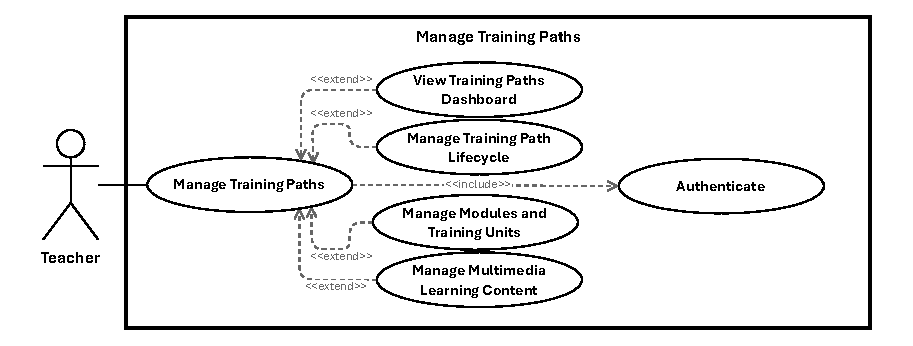
\includegraphics[width=\textwidth]{assets/chapter3/teacher-manage-training-paths-use-case}
    \caption{Use Case Manage Training Paths}
    \label{fig:teacher-manage-training-paths-use-case}
\end{figure}
\dotsection{\textbf{Specification of the Use Case View Training Paths Dashboard}}
\begin{table}[H]
    \centering
    \caption{Use Case Specification: View Training Paths Dashboard}
    \begin{tabular}{|p{3.5cm}|p{10.5cm}|}
        \hline
        \textbf{Title}          & View Training Paths Dashboard \\
        \hline
        \textbf{Summary}        & Teacher views all owned training paths with statistics including total engineers, average ratings, and completion rates \\
        \hline
        \textbf{Actor}          & Teacher \\
        \hline
        \textbf{Precondition}   & Teacher is authenticated, verified, and approved to teach \\
        \hline
        \textbf{Post-condition} & Teacher views the list of owned training paths with key metrics \\
        \hline
        \textbf{Basic Scenario} & \begin{minipage}[t]{\linewidth}
            \begin{enumerate}[topsep=0pt,itemsep=1pt,parsep=0pt,partopsep=0pt]
                \item Teacher navigates to the teaching dashboard
                \item System retrieves all training paths owned by the teacher
                \item System calculates and displays statistics per path
                \item Teacher may click any training path to view or edit details
            \end{enumerate}
        \end{minipage} \\
        \hline
        \textbf{Error Scenario} & \begin{minipage}[t]{\linewidth}
            \begin{enumerate}[topsep=0pt,itemsep=1pt,parsep=0pt,partopsep=0pt]
                \item If no training paths exist, system displays empty state with create option
                \item If teacher is not approved, system redirects to pending approval page
            \end{enumerate}
        \end{minipage} \\
        \hline
    \end{tabular}
    \label{tab:teacher-view-dashboard}
\end{table}
\dotsection{\textbf{Specification of the Use Case Manage Training Path Lifecycle}}
\begin{table}[H]
    \centering
    \caption{Use Case Specification: Manage Training Path Lifecycle}
    \begin{tabular}{|p{3.5cm}|p{10.5cm}|}
        \hline
        \textbf{Title}          & Manage Training Path Lifecycle \\
        \hline
        \textbf{Summary}        & Teacher creates, edits, deletes, archives, restores, and submits training paths for review throughout their lifecycle \\
        \hline
        \textbf{Actor}          & Teacher \\
        \hline
        \textbf{Precondition}   & Teacher is authenticated, verified, approved to teach, and owns the target training path where applicable \\
        \hline
        \textbf{Post-condition} & The training path is created, updated, removed, archived, restored, or submitted for review according to the action performed \\
        \hline
        \textbf{Basic Scenario} & \begin{minipage}[t]{\linewidth}
            \begin{enumerate}[topsep=0pt,itemsep=1pt,parsep=0pt,partopsep=0pt]
                \item Teacher selects a lifecycle action from the dashboard: create, edit, delete, archive, restore, or submit for review
                \item For \textbf{Create}: Teacher fills in title, description, category, price, and difficulty, then submits; system creates the path with draft status
                \item For \textbf{Edit}: Teacher modifies desired metadata fields and submits; system validates and persists changes
                \item For \textbf{Delete}: Teacher confirms permanent deletion; system cascades removal of all associated content
                \item For \textbf{Archive}: Teacher confirms archiving; system soft-deletes the path and removes it from public listings
                \item For \textbf{Restore}: Teacher selects an archived path and confirms restoration; system returns it to its previous state
                \item For \textbf{Submit for Review}: Teacher confirms submission; system transitions the path to pending review and notifies administrators
            \end{enumerate}
        \end{minipage} \\
        \hline
        \textbf{Error Scenario} & \begin{minipage}[t]{\linewidth}
            \begin{enumerate}[topsep=0pt,itemsep=1pt,parsep=0pt,partopsep=0pt]
                \item Missing or invalid fields cause validation failure and surface specific error messages
                \item Deletion is blocked if active enrollments exist
                \item Submission is rejected if the training path is incomplete
                \item Unauthorized actions are denied and access is blocked
                \item Persistence failures preserve the previous state and surface a recoverable error
            \end{enumerate}
        \end{minipage} \\
        \hline
    \end{tabular}
    \label{tab:teacher-tp-lifecycle}
\end{table}
\dotsection{\textbf{Specification of the Use Case Manage Modules and Training Units}}
\begin{table}[H]
    \centering
    \caption{Use Case Specification: Manage Modules and Training Units}
    \begin{tabular}{|p{3.5cm}|p{10.5cm}|}
        \hline
        \textbf{Title}          & Manage Modules and Training Units \\
        \hline
        \textbf{Summary}        & Teacher adds, edits, reorders, and deletes modules and their contained training units to structure the learning content of a training path \\
        \hline
        \textbf{Actor}          & Teacher \\
        \hline
        \textbf{Precondition}   & Teacher is authorized to edit the target training path \\
        \hline
        \textbf{Post-condition} & The training path structure is updated to reflect the added, modified, reordered, or removed modules and training units \\
        \hline
        \textbf{Basic Scenario} & \begin{minipage}[t]{\linewidth}
            \begin{enumerate}[topsep=0pt,itemsep=1pt,parsep=0pt,partopsep=0pt]
                \item Teacher opens the training path editor
                \item Teacher selects an action on a module or training unit: add, edit, reorder, or delete
                \item For \textbf{Add}: Teacher enters title and description and submits; system creates the item and appends it to the structure
                \item For \textbf{Edit}: Teacher modifies desired fields and submits; system validates and persists updates
                \item For \textbf{Reorder}: Teacher drags items to the desired position; system persists the new order
                \item For \textbf{Delete}: Teacher confirms deletion; system removes the item and all contained content with a cascading delete
                \item System reflects all structural changes in the editor view
            \end{enumerate}
        \end{minipage} \\
        \hline
        \textbf{Error Scenario} & \begin{minipage}[t]{\linewidth}
            \begin{enumerate}[topsep=0pt,itemsep=1pt,parsep=0pt,partopsep=0pt]
                \item Missing required fields surface validation errors
                \item Deletion of items with active engineer progress is warned or blocked
                \item Unauthorized access is denied
                \item Persistence failures preserve the previous structure and surface a recoverable error
            \end{enumerate}
        \end{minipage} \\
        \hline
    \end{tabular}
    \label{tab:teacher-modules-units}
\end{table}
\dotsection{\textbf{Specification of the Use Case Manage Multimedia Learning Content}}
\begin{table}[H]
    \centering
    \caption{Use Case Specification: Manage Multimedia Learning Content}
    \begin{tabular}{|p{3.5cm}|p{10.5cm}|}
        \hline
        \textbf{Title}          & Manage Multimedia Learning Content \\
        \hline
        \textbf{Summary}        & Teacher creates or updates articles, videos, captions, and quizzes associated with a training unit \\
        \hline
        \textbf{Actor}          & Teacher \\
        \hline
        \textbf{Precondition}   & Teacher is authorized to edit the target training path and training unit \\
        \hline
        \textbf{Post-condition} & The selected educational asset is created, updated, published, unpublished, or deleted according to the action performed \\
        \hline
        \textbf{Basic Scenario} & \begin{minipage}[t]{\linewidth}
            \begin{enumerate}[topsep=0pt,itemsep=1pt,parsep=0pt,partopsep=0pt]
                \item Teacher selects a training unit and opens the content editor
                \item For \textbf{Article}: Teacher writes or edits rich text content with formatting and media; system persists on save
                \item For \textbf{Video}: Teacher uploads a video file; system validates format and size, stores the file, and queues it for transcoding; Teacher may monitor transcoding status, retry on failure, and manage caption files per language
                \item For \textbf{Quiz}: Teacher creates a quiz with title, passing score, and time limit; adds, reorders, and manages multiple-choice questions with marked correct answers; then publishes or unpublishes the quiz; Teacher may also view attempt statistics including pass rates and average scores
                \item System validates content structure and ownership at each step
                \item System persists the asset and updates the training unit status accordingly
            \end{enumerate}
        \end{minipage} \\
        \hline
        \textbf{Error Scenario} & \begin{minipage}[t]{\linewidth}
            \begin{enumerate}[topsep=0pt,itemsep=1pt,parsep=0pt,partopsep=0pt]
                \item Invalid or incomplete content causes validation failure with specific messages
                \item Unauthorized editing is blocked
                \item Video format or size violations prevent upload
                \item Media processing failure leaves the asset in a retryable state
                \item Quiz publication is blocked if no questions exist
            \end{enumerate}
        \end{minipage} \\
        \hline
    \end{tabular}
    \label{tab:teacher-content}
\end{table}


\iffalse
% ------------------------------------------------------------------
% 1. Manage Training Path
% ------------------------------------------------------------------
\dotsection{\textbf{Specification of the Use Case Manage Training Path}}
\begin{table}[H]
    \centering
    \caption{Use Case Specification: Manage Training Path}
    \begin{tabular}{|p{3.5cm}|p{10.5cm}|}
        \hline
        \textbf{Title}          & Manage Training Path \\
        \hline
        \textbf{Summary}        & Teacher performs lifecycle operations on training paths: view dashboard with statistics, create, edit details, delete, archive, restore, and submit for admin review \\
        \hline
        \textbf{Actor}          & Teacher \\
        \hline
        \textbf{Covered Operations} & View Dashboard, Create, Edit Details, Delete, Archive, Restore, Submit for Review \\
        \hline
        \textbf{Precondition}   & Teacher is authenticated, verified, and approved to teach; for ownership-scoped operations the teacher must own the target training path \\
        \hline
        \textbf{Post-condition} & The requested operation is applied: path is created / updated / deleted / archived / restored / submitted, and the dashboard reflects the new state \\
        \hline
        \textbf{Basic Scenario} &
        \begin{minipage}[t]{\linewidth}
            \begin{enumerate}[topsep=0pt,itemsep=1pt,parsep=0pt,partopsep=0pt]
                \item Teacher navigates to the teaching dashboard; system retrieves all owned training paths with statistics (total engineers, average rating, completion rate).
                \item \textbf{Create:} Teacher clicks ``Create New Training Path'', fills in title, description, category, price, and difficulty level, then submits; system creates the path with \textit{draft} status and redirects to the editor.
                \item \textbf{Edit Details:} Teacher opens a path, modifies desired metadata fields, and submits; system validates and persists the changes.
                \item \textbf{Delete:} Teacher selects a path, confirms the deletion dialog; system cascades deletion of all modules, units, and content.
                \item \textbf{Archive:} Teacher confirms the archive dialog; system soft-deletes the path, removing it from public listings while preserving all data.
                \item \textbf{Restore:} Teacher navigates to the archived section, selects a path, confirms restoration; system reverts the soft-delete and re-exposes the path.
                \item \textbf{Submit for Review:} Teacher completes required structure and invokes submit; system transitions path status to \textit{pending review} and makes it visible in the admin approval dashboard.
            \end{enumerate}
        \end{minipage} \\
        \hline
        \textbf{Error Scenarios} &
        \begin{minipage}[t]{\linewidth}
            \begin{enumerate}[topsep=0pt,itemsep=1pt,parsep=0pt,partopsep=0pt]
                \item Missing required fields on create/edit → system displays validation errors and preserves input.
                \item Teacher does not own the target path → system denies access for all write operations.
                \item Delete attempted on a path with active enrollments → system prevents deletion.
                \item Submit attempted on an incomplete path → system rejects submission with details.
                \item Rate limit exceeded on create → system displays throttle warning.
                \item Any persistence failure → system preserves the previous state and logs the error.
                \item Teacher not yet approved → system redirects to pending-approval page.
                \item Empty dashboard (no paths exist) → system displays empty state with create option.
            \end{enumerate}
        \end{minipage} \\
        \hline
    \end{tabular}
    \label{tab:teacher-manage-tp}
\end{table}
 
% ------------------------------------------------------------------
% 2. Manage Modules
% ------------------------------------------------------------------
\dotsection{\textbf{Specification of the Use Case Manage Modules}}
\begin{table}[H]
    \centering
    \caption{Use Case Specification: Manage Modules}
    \begin{tabular}{|p{3.5cm}|p{10.5cm}|}
        \hline
        \textbf{Title}          & Manage Modules \\
        \hline
        \textbf{Summary}        & Teacher adds, edits, reorders, and deletes modules within a training path to organise the learning structure \\
        \hline
        \textbf{Actor}          & Teacher \\
        \hline
        \textbf{Covered Operations} & Add Module, Edit Module, Reorder Modules, Delete Module \\
        \hline
        \textbf{Precondition}   & Teacher owns the training path and is in edit mode; reorder requires at least two modules \\
        \hline
        \textbf{Post-condition} & Module structure of the training path reflects the applied operation \\
        \hline
        \textbf{Basic Scenario} &
        \begin{minipage}[t]{\linewidth}
            \begin{enumerate}[topsep=0pt,itemsep=1pt,parsep=0pt,partopsep=0pt]
                \item Teacher opens the training path editor; system displays the current module list.
                \item \textbf{Add:} Teacher clicks ``Add Module'', enters title and description, and submits; system creates the module and appends it to the path.
                \item \textbf{Edit:} Teacher selects a module, modifies the title or description in the edit form, and submits; system validates and persists the update.
                \item \textbf{Reorder:} Teacher drags and drops modules into the desired sequence; system updates and persists the new order positions.
                \item \textbf{Delete:} Teacher selects a module and confirms the deletion dialog (which warns about contained units); system removes the module and all its training units, then refreshes the list.
            \end{enumerate}
        \end{minipage} \\
        \hline
        \textbf{Error Scenarios} &
        \begin{minipage}[t]{\linewidth}
            \begin{enumerate}[topsep=0pt,itemsep=1pt,parsep=0pt,partopsep=0pt]
                \item Teacher does not own the training path → system denies access.
                \item Required fields missing on add/edit → system displays validation errors.
                \item Module has active engineer progress on delete → system warns or prevents deletion.
                \item Reorder or persistence failure → system displays error and preserves the previous order/state.
            \end{enumerate}
        \end{minipage} \\
        \hline
    \end{tabular}
    \label{tab:teacher-manage-modules}
\end{table}
 
% ------------------------------------------------------------------
% 3. Manage Training Units
% ------------------------------------------------------------------
\dotsection{\textbf{Specification of the Use Case Manage Training Units}}
\begin{table}[H]
    \centering
    \caption{Use Case Specification: Manage Training Units}
    \begin{tabular}{|p{3.5cm}|p{10.5cm}|}
        \hline
        \textbf{Title}          & Manage Training Units \\
        \hline
        \textbf{Summary}        & Teacher adds, edits, reorders, and deletes training units inside a module to define the granular learning sequence \\
        \hline
        \textbf{Actor}          & Teacher \\
        \hline
        \textbf{Covered Operations} & Add Training Unit, Edit Training Unit, Reorder Units, Delete Training Unit \\
        \hline
        \textbf{Precondition}   & Teacher owns the training path and the target module exists; reorder requires at least two units \\
        \hline
        \textbf{Post-condition} & The module's unit list reflects the applied operation \\
        \hline
        \textbf{Basic Scenario} &
        \begin{minipage}[t]{\linewidth}
            \begin{enumerate}[topsep=0pt,itemsep=1pt,parsep=0pt,partopsep=0pt]
                \item Teacher opens the training path editor and selects a module.
                \item \textbf{Add:} Teacher clicks ``Add Training Unit'', enters title, description, and content type, and submits; system creates the unit and appends it to the module.
                \item \textbf{Edit:} Teacher selects a unit, modifies desired fields in the edit form, and submits; system validates and persists the update.
                \item \textbf{Reorder:} Teacher drags and drops units into the desired sequence; system updates and persists the new order positions.
                \item \textbf{Delete:} Teacher selects a unit and confirms the deletion dialog (which warns about associated content); system removes the unit and all its content, then refreshes the module view.
            \end{enumerate}
        \end{minipage} \\
        \hline
        \textbf{Error Scenarios} &
        \begin{minipage}[t]{\linewidth}
            \begin{enumerate}[topsep=0pt,itemsep=1pt,parsep=0pt,partopsep=0pt]
                \item Teacher does not own the training path → system denies access.
                \item Required fields missing on add/edit → system displays validation errors.
                \item Unit has active engineer progress on delete → system warns or prevents deletion.
                \item Reorder or persistence failure → system displays error and preserves the previous order/state.
            \end{enumerate}
        \end{minipage} \\
        \hline
    \end{tabular}
    \label{tab:teacher-manage-units}
\end{table}
 
% ------------------------------------------------------------------
% 4. Manage Quiz
% ------------------------------------------------------------------
\dotsection{\textbf{Specification of the Use Case Manage Quiz}}
\begin{table}[H]
    \centering
    \caption{Use Case Specification: Manage Quiz}
    \begin{tabular}{|p{3.5cm}|p{10.5cm}|}
        \hline
        \textbf{Title}          & Manage Quiz \\
        \hline
        \textbf{Summary}        & Teacher creates, configures, publishes/unpublishes, and deletes the quiz associated with a training unit \\
        \hline
        \textbf{Actor}          & Teacher \\
        \hline
        \textbf{Covered Operations} & Create Quiz, Edit Quiz Settings, Publish / Unpublish Quiz, Delete Quiz \\
        \hline
        \textbf{Precondition}   & Teacher owns the training path and the target training unit exists; publishing requires at least one question \\
        \hline
        \textbf{Post-condition} & Quiz is created / updated / published / unpublished / deleted and its visibility to engineers changes accordingly \\
        \hline
        \textbf{Basic Scenario} &
        \begin{minipage}[t]{\linewidth}
            \begin{enumerate}[topsep=0pt,itemsep=1pt,parsep=0pt,partopsep=0pt]
                \item Teacher opens the training unit editor and navigates to the quiz section.
                \item \textbf{Create:} Teacher clicks ``Create Quiz'', fills in title, description, passing score, and time limit, and submits; system creates the quiz with \textit{unpublished} status.
                \item \textbf{Edit Settings:} Teacher opens the existing quiz, modifies configuration fields, and submits; system validates and persists the changes.
                \item \textbf{Publish:} Teacher clicks ``Publish''; system validates that at least one question exists, updates the status, and makes the quiz visible to enrolled engineers.
                \item \textbf{Unpublish:} Teacher clicks ``Unpublish''; system hides the quiz from engineers while preserving all data.
                \item \textbf{Delete:} Teacher confirms the deletion dialog; system removes the quiz and all associated questions and attempts.
            \end{enumerate}
        \end{minipage} \\
        \hline
        \textbf{Error Scenarios} &
        \begin{minipage}[t]{\linewidth}
            \begin{enumerate}[topsep=0pt,itemsep=1pt,parsep=0pt,partopsep=0pt]
                \item Teacher does not own the training path → system denies access.
                \item Quiz already exists for the unit on create → system displays error.
                \item Publish attempted with no questions → system prevents publication.
                \item Validation failure on settings edit → system displays specific errors and preserves previous state.
                \item Any persistence failure → system preserves previous state and displays error.
            \end{enumerate}
        \end{minipage} \\
        \hline
    \end{tabular}
    \label{tab:teacher-manage-quiz}
\end{table}
 
% ------------------------------------------------------------------
% 5. Manage Quiz Questions
% ------------------------------------------------------------------
\dotsection{\textbf{Specification of the Use Case Manage Quiz Questions}}
\begin{table}[H]
    \centering
    \caption{Use Case Specification: Manage Quiz Questions}
    \begin{tabular}{|p{3.5cm}|p{10.5cm}|}
        \hline
        \textbf{Title}          & Manage Quiz Questions \\
        \hline
        \textbf{Summary}        & Teacher adds questions with multiple-choice options and reorders them within a quiz \\
        \hline
        \textbf{Actor}          & Teacher \\
        \hline
        \textbf{Covered Operations} & Add Questions \& Options, Reorder Questions \\
        \hline
        \textbf{Precondition}   & Teacher owns the training path and a quiz exists for the target training unit; reorder requires at least two questions \\
        \hline
        \textbf{Post-condition} & Quiz question list reflects the new question(s) or updated order \\
        \hline
        \textbf{Basic Scenario} &
        \begin{minipage}[t]{\linewidth}
            \begin{enumerate}[topsep=0pt,itemsep=1pt,parsep=0pt,partopsep=0pt]
                \item Teacher opens the quiz editor; system displays the current question list.
                \item \textbf{Add:} Teacher clicks ``Add Question'', enters question text, type, and multiple-choice options, marks the correct answer, and submits; system creates the question and appends it to the quiz.
                \item \textbf{Reorder:} Teacher drags and drops questions into the desired sequence; system updates and persists the new order positions.
            \end{enumerate}
        \end{minipage} \\
        \hline
        \textbf{Error Scenarios} &
        \begin{minipage}[t]{\linewidth}
            \begin{enumerate}[topsep=0pt,itemsep=1pt,parsep=0pt,partopsep=0pt]
                \item Teacher does not own the training path → system denies access.
                \item Required fields missing on add → system displays validation errors.
                \item No correct answer marked → system displays error and blocks submission.
                \item Reorder or persistence failure → system displays error and preserves the previous order.
            \end{enumerate}
        \end{minipage} \\
        \hline
    \end{tabular}
    \label{tab:teacher-manage-questions}
\end{table}
 
% ------------------------------------------------------------------
% 6. View Quiz Statistics
% ------------------------------------------------------------------
\dotsection{\textbf{Specification of the Use Case View Quiz Statistics}}
\begin{table}[H]
    \centering
    \caption{Use Case Specification: View Quiz Statistics}
    \begin{tabular}{|p{3.5cm}|p{10.5cm}|}
        \hline
        \textbf{Title}          & View Quiz Statistics \\
        \hline
        \textbf{Summary}        & Teacher views quiz performance data including attempt counts, pass rates, average scores, and per-question analytics \\
        \hline
        \textbf{Actor}          & Teacher \\
        \hline
        \textbf{Precondition}   & Teacher owns the training path and the quiz has at least one engineer attempt \\
        \hline
        \textbf{Post-condition} & Teacher views comprehensive quiz statistics and performance metrics \\
        \hline
        \textbf{Basic Scenario} &
        \begin{minipage}[t]{\linewidth}
            \begin{enumerate}[topsep=0pt,itemsep=1pt,parsep=0pt,partopsep=0pt]
                \item Teacher opens the quiz editor and navigates to the statistics section.
                \item System retrieves attempt data and displays total attempts, pass rate, and average score.
                \item System shows question-level performance data.
                \item Teacher may filter results by date range or engineer group.
            \end{enumerate}
        \end{minipage} \\
        \hline
        \textbf{Error Scenarios} &
        \begin{minipage}[t]{\linewidth}
            \begin{enumerate}[topsep=0pt,itemsep=1pt,parsep=0pt,partopsep=0pt]
                \item Teacher does not own the training path → system denies access.
                \item No attempts exist yet → system displays an empty-state message.
            \end{enumerate}
        \end{minipage} \\
        \hline
    \end{tabular}
    \label{tab:teacher-quiz-stats}
\end{table}
 
% ------------------------------------------------------------------
% 7. Manage Article Content
% ------------------------------------------------------------------
\dotsection{\textbf{Specification of the Use Case Manage Article Content}}
\begin{table}[H]
    \centering
    \caption{Use Case Specification: Manage Article Content}
    \begin{tabular}{|p{3.5cm}|p{10.5cm}|}
        \hline
        \textbf{Title}          & Manage Article Content \\
        \hline
        \textbf{Summary}        & Teacher creates, updates, and deletes rich-text article content for a training unit \\
        \hline
        \textbf{Actor}          & Teacher \\
        \hline
        \textbf{Covered Operations} & Create / Update Article Content, Delete Article \\
        \hline
        \textbf{Precondition}   & Teacher owns the training path and the target training unit exists; delete requires an article to already exist \\
        \hline
        \textbf{Post-condition} & Article content is created, updated, or removed from the training unit \\
        \hline
        \textbf{Basic Scenario} &
        \begin{minipage}[t]{\linewidth}
            \begin{enumerate}[topsep=0pt,itemsep=1pt,parsep=0pt,partopsep=0pt]
                \item Teacher opens the training unit editor and navigates to the article section.
                \item \textbf{Create / Update:} System displays the rich-text editor with any existing content; teacher writes or edits content (text, images, links, media) and saves; system persists the content and confirms the save.
                \item \textbf{Delete:} Teacher clicks delete article, confirms the dialog; system removes the article content, confirms deletion, and clears the editor.
            \end{enumerate}
        \end{minipage} \\
        \hline
        \textbf{Error Scenarios} &
        \begin{minipage}[t]{\linewidth}
            \begin{enumerate}[topsep=0pt,itemsep=1pt,parsep=0pt,partopsep=0pt]
                \item Teacher does not own the training path → system denies access.
                \item Content exceeds size limits → system displays an error.
                \item Delete attempted when no article exists → system displays not-found error.
                \item Save or deletion failure → system displays error and may preserve draft state.
            \end{enumerate}
        \end{minipage} \\
        \hline
    \end{tabular}
    \label{tab:teacher-manage-article}
\end{table}
 
% ------------------------------------------------------------------
% 8. Manage Video Content
% ------------------------------------------------------------------
\dotsection{\textbf{Specification of the Use Case Manage Video Content}}
\begin{table}[H]
    \centering
    \caption{Use Case Specification: Manage Video Content}
    \begin{tabular}{|p{3.5cm}|p{10.5cm}|}
        \hline
        \textbf{Title}          & Manage Video Content \\
        \hline
        \textbf{Summary}        & Teacher uploads a video, monitors its transcoding progress, retries failed processing, and manages caption/subtitle files for accessibility \\
        \hline
        \textbf{Actor}          & Teacher \\
        \hline
        \textbf{Covered Operations} & Upload Video, Monitor Transcoding Status, Retry Failed Processing, Manage Captions / Subtitles \\
        \hline
        \textbf{Precondition}   & Teacher owns the training path and the target training unit exists; retry requires a video in \textit{failed} state; caption management requires a fully processed video \\
        \hline
        \textbf{Post-condition} & Video is uploaded and queued, processing status is visible, failed jobs are requeued, and caption files are associated with the video and available to engineers \\
        \hline
        \textbf{Basic Scenario} &
        \begin{minipage}[t]{\linewidth}
            \begin{enumerate}[topsep=0pt,itemsep=1pt,parsep=0pt,partopsep=0pt]
                \item Teacher opens the training unit editor and navigates to the video section.
                \item \textbf{Upload:} Teacher selects a video file; system validates format and size, uploads the file to storage, queues it for transcoding, and displays the processing status.
                \item \textbf{Monitor Transcoding:} System displays progress percentage and current processing stage; upon completion it lists available quality levels; teacher may refresh or receive notifications.
                \item \textbf{Retry Failed Processing:} When transcoding has failed, teacher clicks ``Retry Transcoding''; system validates the failed state, requeues the video, and displays the new processing status.
                \item \textbf{Manage Captions:} System displays existing caption files with their languages; teacher selects a caption file, specifies language and label, and uploads it; teacher may also delete existing captions; system updates the caption list after each operation.
            \end{enumerate}
        \end{minipage} \\
        \hline
        \textbf{Error Scenarios} &
        \begin{minipage}[t]{\linewidth}
            \begin{enumerate}[topsep=0pt,itemsep=1pt,parsep=0pt,partopsep=0pt]
                \item Teacher does not own the training path → system denies access.
                \item Invalid video format or file exceeds size limit → system displays error before upload begins.
                \item Upload or transcoding failure → system displays error with retry option.
                \item Retry attempted when video is not in failed state → system displays error.
                \item Invalid caption file format or upload failure → system displays error with retry option.
                \item Video not found → system displays not-found error.
            \end{enumerate}
        \end{minipage} \\
        \hline
    \end{tabular}
    \label{tab:teacher-manage-video}
\end{table}
\fi

\iffalse
\dotsection{\textbf{Specification of the Use Case View Training Paths Dashboard}}
\begin{table}[H]
    \centering
    \caption{Use Case Specification: View Training Paths Dashboard}
    \begin{tabular}{|p{3.5cm}|p{10.5cm}|}
        \hline
        \textbf{Title}          & View Training Paths Dashboard                                                                 \\
        \hline
        \textbf{Summary}        & Teacher views their training paths with statistics including total engineers, average ratings, and completion rates \\
        \hline
        \textbf{Actor}          & Teacher                                                                                      \\
        \hline
        \textbf{Precondition}   & Teacher is authenticated, verified, and approved to teach                                     \\
        \hline
        \textbf{Post-condition} & Teacher views list of owned training paths with key metrics                                   \\
        \hline
        \textbf{Basic Scenario} & \begin{minipage}[t]{\linewidth}
                                      \begin{enumerate}[topsep=0pt,itemsep=1pt,parsep=0pt,partopsep=0pt]
                                          \item Teacher navigates to the teaching dashboard
                                          \item System retrieves all training paths owned by the teacher
                                          \item System calculates statistics: total engineers, average rating, completion rate
                                          \item System displays training paths with titles, status, and metrics
                                          \item Teacher may click on any training path to view or edit details
                                      \end{enumerate}
                                  \end{minipage} \\
        \hline
        \textbf{Error Scenario} & \begin{minipage}[t]{\linewidth}
                                      \begin{enumerate}[topsep=0pt,itemsep=1pt,parsep=0pt,partopsep=0pt]
                                          \item If no training paths exist, system displays empty state with create option
                                          \item If teacher is not approved, system redirects to pending approval page
                                      \end{enumerate}
                                  \end{minipage} \\
        \hline
    \end{tabular}
    \label{tab:teacher-view-dashboard}
\end{table}
\dotsection{\textbf{Specification of the Use Case Create Training Path}}
\begin{table}[H]
    \centering
    \caption{Use Case Specification: Create Training Path}
    \begin{tabular}{|p{3.5cm}|p{10.5cm}|}
        \hline
        \textbf{Title}          & Create Training Path                                                                 \\
        \hline
        \textbf{Summary}        & Teacher creates a new training path with title, description, category, pricing, and initial structure \\
        \hline
        \textbf{Actor}          & Teacher                                                                              \\
        \hline
        \textbf{Precondition}   & Teacher is authenticated, verified, and approved to teach                                 \\
        \hline
        \textbf{Post-condition} & A new training path is created with draft status and assigned to the teacher            \\
        \hline
        \textbf{Basic Scenario} & \begin{minipage}[t]{\linewidth}
                                      \begin{enumerate}[topsep=0pt,itemsep=1pt,parsep=0pt,partopsep=0pt]
                                          \item Teacher clicks "Create New Training Path" from dashboard
                                          \item System displays creation form with available categories and VM templates
                                          \item Teacher enters title, description, category, price, and difficulty level
                                          \item Teacher may optionally add initial modules and training units
                                          \item Teacher submits the form
                                          \item System validates input and creates training path with draft status
                                          \item System redirects to edit page for content addition
                                      \end{enumerate}
                                  \end{minipage} \\
        \hline
        \textbf{Error Scenario} & \begin{minipage}[t]{\linewidth}
                                      \begin{enumerate}[topsep=0pt,itemsep=1pt,parsep=0pt,partopsep=0pt]
                                          \item If required fields are missing, system displays validation errors
                                          \item If rate limit exceeded, system displays throttle warning
                                          \item If creation fails, system preserves input and shows error message
                                      \end{enumerate}
                                  \end{minipage} \\
        \hline
    \end{tabular}
    \label{tab:teacher-create-tp}
\end{table}
\dotsection{\textbf{Specification of the Use Case Edit Training Path Details}}
\begin{table}[H]
    \centering
    \caption{Use Case Specification: Edit Training Path Details}
    \begin{tabular}{|p{3.5cm}|p{10.5cm}|}
        \hline
        \textbf{Title}          & Edit Training Path Details                                                                 \\
        \hline
        \textbf{Summary}        & Teacher modifies training path metadata including title, description, category, and pricing \\
        \hline
        \textbf{Actor}          & Teacher                                                                              \\
        \hline
        \textbf{Precondition}   & Teacher owns the training path and it is not in published state without admin approval \\
        \hline
        \textbf{Post-condition} & Training path details are updated in the system                                          \\
        \hline
        \textbf{Basic Scenario} & \begin{minipage}[t]{\linewidth}
                                      \begin{enumerate}[topsep=0pt,itemsep=1pt,parsep=0pt,partopsep=0pt]
                                          \item Teacher opens training path from dashboard
                                          \item System displays edit form with current values
                                          \item Teacher modifies desired fields (title, description, category, price, etc.)
                                          \item Teacher submits changes
                                          \item System validates updates and persists changes
                                          \item System confirms successful update
                                      \end{enumerate}
                                  \end{minipage} \\
        \hline
        \textbf{Error Scenario} & \begin{minipage}[t]{\linewidth}
                                      \begin{enumerate}[topsep=0pt,itemsep=1pt,parsep=0pt,partopsep=0pt]
                                          \item If teacher does not own training path, system denies access
                                          \item If validation fails, system displays specific error messages
                                          \item If update fails, system preserves previous state
                                      \end{enumerate}
                                  \end{minipage} \\
        \hline
    \end{tabular}
    \label{tab:teacher-edit-tp}
\end{table}
\dotsection{\textbf{Specification of the Use Case Delete Training Path}}
\begin{table}[H]
    \centering
    \caption{Use Case Specification: Delete Training Path}
    \begin{tabular}{|p{3.5cm}|p{10.5cm}|}
        \hline
        \textbf{Title}          & Delete Training Path                                                                 \\
        \hline
        \textbf{Summary}        & Teacher permanently deletes a training path and all associated content               \\
        \hline
        \textbf{Actor}          & Teacher                                                                              \\
        \hline
        \textbf{Precondition}   & Teacher owns the training path and it has no active enrollments                       \\
        \hline
        \textbf{Post-condition} & Training path and all related data are permanently removed from the system           \\
        \hline
        \textbf{Basic Scenario} & \begin{minipage}[t]{\linewidth}
                                      \begin{enumerate}[topsep=0pt,itemsep=1pt,parsep=0pt,partopsep=0pt]
                                          \item Teacher selects training path from dashboard
                                          \item Teacher clicks delete option
                                          \item System displays confirmation dialog with warning
                                          \item Teacher confirms deletion
                                          \item System performs cascading delete of training path, modules, units, and content
                                          \item System confirms successful deletion and removes from list
                                      \end{enumerate}
                                  \end{minipage} \\
        \hline
        \textbf{Error Scenario} & \begin{minipage}[t]{\linewidth}
                                      \begin{enumerate}[topsep=0pt,itemsep=1pt,parsep=0pt,partopsep=0pt]
                                          \item If training path has active enrollments, system prevents deletion
                                          \item If teacher does not own training path, system denies access
                                          \item If deletion fails, system displays error and preserves data
                                      \end{enumerate}
                                  \end{minipage} \\
        \hline
    \end{tabular}
    \label{tab:teacher-delete-tp}
\end{table}
\dotsection{\textbf{Specification of the Use Case Archive Training Path}}
\begin{table}[H]
    \centering
    \caption{Use Case Specification: Archive Training Path}
    \begin{tabular}{|p{3.5cm}|p{10.5cm}|}
        \hline
        \textbf{Title}          & Archive Training Path                                                                 \\
        \hline
        \textbf{Summary}        & Teacher archives a training path to hide it from public view while preserving data for potential restoration \\
        \hline
        \textbf{Actor}          & Teacher                                                                              \\
        \hline
        \textbf{Precondition}   & Teacher owns the training path                                                       \\
        \hline
        \textbf{Post-condition} & Training path is soft-deleted and removed from public listings                       \\
        \hline
        \textbf{Basic Scenario} & \begin{minipage}[t]{\linewidth}
                                      \begin{enumerate}[topsep=0pt,itemsep=1pt,parsep=0pt,partopsep=0pt]
                                          \item Teacher selects training path from dashboard
                                          \item Teacher clicks archive option
                                          \item System displays confirmation dialog
                                          \item Teacher confirms archiving
                                          \item System performs soft delete, preserving all data
                                          \item System removes training path from public view and active listings
                                      \end{enumerate}
                                  \end{minipage} \\
        \hline
        \textbf{Error Scenario} & \begin{minipage}[t]{\linewidth}
                                      \begin{enumerate}[topsep=0pt,itemsep=1pt,parsep=0pt,partopsep=0pt]
                                          \item If teacher does not own training path, system denies access
                                          \item If archiving fails, system displays error and preserves current state
                                      \end{enumerate}
                                  \end{minipage} \\
        \hline
    \end{tabular}
    \label{tab:teacher-archive-tp}
\end{table}
\dotsection{\textbf{Specification of the Use Case Restore Archived Path}}
\begin{table}[H]
    \centering
    \caption{Use Case Specification: Restore Archived Path}
    \begin{tabular}{|p{3.5cm}|p{10.5cm}|}
        \hline
        \textbf{Title}          & Restore Archived Path                                                                 \\
        \hline
        \textbf{Summary}        & Teacher restores a previously archived training path to make it available again         \\
        \hline
        \textbf{Actor}          & Teacher                                                                              \\
        \hline
        \textbf{Precondition}   & Teacher owns the archived training path                                              \\
        \hline
        \textbf{Post-condition} & Training path is restored to its previous state and becomes visible again             \\
        \hline
        \textbf{Basic Scenario} & \begin{minipage}[t]{\linewidth}
                                      \begin{enumerate}[topsep=0pt,itemsep=1pt,parsep=0pt,partopsep=0pt]
                                          \item Teacher navigates to archived training paths section
                                          \item Teacher selects archived training path to restore
                                          \item Teacher clicks restore option
                                          \item System displays confirmation dialog
                                          \item Teacher confirms restoration
                                          \item System restores training path to its previous state
                                          \item Training path becomes visible in dashboard and public listings
                                      \end{enumerate}
                                  \end{minipage} \\
        \hline
        \textbf{Error Scenario} & \begin{minipage}[t]{\linewidth}
                                      \begin{enumerate}[topsep=0pt,itemsep=1pt,parsep=0pt,partopsep=0pt]
                                          \item If teacher does not own training path, system denies access
                                          \item If restoration fails, system displays error and preserves archived state
                                      \end{enumerate}
                                  \end{minipage} \\
        \hline
    \end{tabular}
    \label{tab:teacher-restore-tp}
\end{table}
\dotsection{\textbf{Specification of the Use Case Submit Path for Review}}
\begin{table}[H]
    \centering
    \caption{Use Case Specification: Submit Path for Review}
    \begin{tabular}{|p{3.5cm}|p{10.5cm}|}
        \hline
        \textbf{Title}          & Submit Path for Review                                                                                       \\
        \hline
        \textbf{Summary}        & Teacher submits an authored training path to the administrative workflow for validation and publication readiness     \\
        \hline
        \textbf{Actor}          & Teacher                                                                                                               \\
        \hline
        \textbf{Precondition}   & Teacher is authenticated, verified, approved to teach, and owns the training path                                     \\
        \hline
        \textbf{Post-condition} & The training path status changes to a review-oriented state and becomes visible to administrative approval interfaces \\
        \hline
        \textbf{Basic Scenario} &
        \begin{minipage}[t]{\linewidth}
            \begin{enumerate}[topsep=0pt,itemsep=1pt,parsep=0pt,partopsep=0pt]
                \item Teacher opens the training path management dashboard
                \item Teacher completes the required structure, modules, and training units
                \item Teacher invokes the submit action
                \item System validates ownership and submission eligibility
                \item System updates the training path state to pending review
                \item Administrators can then inspect the submitted training path from the approval
                      dashboard
            \end{enumerate}
        \end{minipage}                                                      \\
        \hline
        \textbf{Error Scenario} &
        \begin{minipage}[t]{\linewidth}
            \begin{enumerate}[topsep=0pt,itemsep=1pt,parsep=0pt,partopsep=0pt]
                \item If the training path is incomplete, the system rejects submission
                \item If the teacher lacks permission, the action is denied
                \item If persistence fails, the previous state is preserved and the failure is logged
            \end{enumerate}
        \end{minipage}                                                    \\
        \hline
    \end{tabular}
    \label{tab:teacher-submit-review}
\end{table}
\dotsection{\textbf{Specification of the Use Case Add Module}}
\begin{table}[H]
    \centering
    \caption{Use Case Specification: Add Module}
    \begin{tabular}{|p{3.5cm}|p{10.5cm}|}
        \hline
        \textbf{Title}          & Add Module                                                                 \\
        \hline
        \textbf{Summary}        & Teacher adds a new module to organize training units within a training path         \\
        \hline
        \textbf{Actor}          & Teacher                                                                      \\
        \hline
        \textbf{Precondition}   & Teacher owns the training path and is in edit mode                              \\
        \hline
        \textbf{Post-condition} & A new module is created and added to the training path structure               \\
        \hline
        \textbf{Basic Scenario} & \begin{minipage}[t]{\linewidth}
                                      \begin{enumerate}[topsep=0pt,itemsep=1pt,parsep=0pt,partopsep=0pt]
                                          \item Teacher opens training path editor
                                          \item Teacher clicks "Add Module" button
                                          \item System displays module creation form
                                          \item Teacher enters module title and description
                                          \item Teacher submits the form
                                          \item System creates module and adds it to training path
                                          \item System updates module list display
                                      \end{enumerate}
                                  \end{minipage} \\
        \hline
        \textbf{Error Scenario} & \begin{minipage}[t]{\linewidth}
                                      \begin{enumerate}[topsep=0pt,itemsep=1pt,parsep=0pt,partopsep=0pt]
                                          \item If required fields are missing, system displays validation errors
                                          \item If teacher does not own training path, system denies access
                                          \item If creation fails, system displays error message
                                      \end{enumerate}
                                  \end{minipage} \\
        \hline
    \end{tabular}
    \label{tab:teacher-add-module}
\end{table}
\dotsection{\textbf{Specification of the Use Case Reorder Modules}}
\begin{table}[H]
    \centering
    \caption{Use Case Specification: Reorder Modules}
    \begin{tabular}{|p{3.5cm}|p{10.5cm}|}
        \hline
        \textbf{Title}          & Reorder Modules                                                                 \\
        \hline
        \textbf{Summary}        & Teacher changes the order of modules within a training path to organize learning flow \\
        \hline
        \textbf{Actor}          & Teacher                                                                      \\
        \hline
        \textbf{Precondition}   & Teacher owns the training path and it has at least two modules                 \\
        \hline
        \textbf{Post-condition} & Module order is updated and reflected in the training path structure           \\
        \hline
        \textbf{Basic Scenario} & \begin{minipage}[t]{\linewidth}
                                      \begin{enumerate}[topsep=0pt,itemsep=1pt,parsep=0pt,partopsep=0pt]
                                          \item Teacher opens training path editor
                                          \item Teacher drags and drops modules to desired order
                                          \item System updates module order positions
                                          \item System persists new order
                                          \item System displays updated module list
                                      \end{enumerate}
                                  \end{minipage} \\
        \hline
        \textbf{Error Scenario} & \begin{minipage}[t]{\linewidth}
                                      \begin{enumerate}[topsep=0pt,itemsep=1pt,parsep=0pt,partopsep=0pt]
                                          \item If teacher does not own training path, system denies access
                                          \item If reordering fails, system displays error and preserves previous order
                                      \end{enumerate}
                                  \end{minipage} \\
        \hline
    \end{tabular}
    \label{tab:teacher-reorder-modules}
\end{table}
\dotsection{\textbf{Specification of the Use Case Delete Module}}
\begin{table}[H]
    \centering
    \caption{Use Case Specification: Delete Module}
    \begin{tabular}{|p{3.5cm}|p{10.5cm}|}
        \hline
        \textbf{Title}          & Delete Module                                                                 \\
        \hline
        \textbf{Summary}        & Teacher removes a module and all its training units from the training path      \\
        \hline
        \textbf{Actor}          & Teacher                                                                      \\
        \hline
        \textbf{Precondition}   & Teacher owns the training path and module is not required for completion        \\
        \hline
        \textbf{Post-condition} & Module and all contained training units are removed from the training path     \\
        \hline
        \textbf{Basic Scenario} & \begin{minipage}[t]{\linewidth}
                                      \begin{enumerate}[topsep=0pt,itemsep=1pt,parsep=0pt,partopsep=0pt]
                                          \item Teacher opens training path editor
                                          \item Teacher selects module to delete
                                          \item Teacher clicks delete option
                                          \item System displays confirmation dialog with warning about contained units
                                          \item Teacher confirms deletion
                                          \item System removes module and all training units
                                          \item System updates training path structure
                                      \end{enumerate}
                                  \end{minipage} \\
        \hline
        \textbf{Error Scenario} & \begin{minipage}[t]{\linewidth}
                                      \begin{enumerate}[topsep=0pt,itemsep=1pt,parsep=0pt,partopsep=0pt]
                                          \item If teacher does not own training path, system denies access
                                          \item If module has active engineer progress, system may warn or prevent deletion
                                          \item If deletion fails, system displays error and preserves data
                                      \end{enumerate}
                                  \end{minipage} \\
        \hline
    \end{tabular}
    \label{tab:teacher-delete-module}
\end{table}
\dotsection{\textbf{Specification of the Use Case Edit Module}}
\begin{table}[H]
    \centering
    \caption{Use Case Specification: Edit Module}
    \begin{tabular}{|p{3.5cm}|p{10.5cm}|}
        \hline
        \textbf{Title}          & Edit Module                                                                 \\
        \hline
        \textbf{Summary}        & Teacher modifies module title, description, and other properties                 \\
        \hline
        \textbf{Actor}          & Teacher                                                                      \\
        \hline
        \textbf{Precondition}   & Teacher owns the training path containing the module                          \\
        \hline
        \textbf{Post-condition} & Module details are updated in the system                                      \\
        \hline
        \textbf{Basic Scenario} & \begin{minipage}[t]{\linewidth}
                                      \begin{enumerate}[topsep=0pt,itemsep=1pt,parsep=0pt,partopsep=0pt]
                                          \item Teacher opens training path editor
                                          \item Teacher selects module to edit
                                          \item System displays module edit form with current values
                                          \item Teacher modifies desired fields
                                          \item Teacher submits changes
                                          \item System validates and persists updates
                                          \item System confirms successful update
                                      \end{enumerate}
                                  \end{minipage} \\
        \hline
        \textbf{Error Scenario} & \begin{minipage}[t]{\linewidth}
                                      \begin{enumerate}[topsep=0pt,itemsep=1pt,parsep=0pt,partopsep=0pt]
                                          \item If teacher does not own training path, system denies access
                                          \item If validation fails, system displays specific errors
                                          \item If update fails, system preserves previous state
                                      \end{enumerate}
                                  \end{minipage} \\
        \hline
    \end{tabular}
    \label{tab:teacher-edit-module}
\end{table}
\dotsection{\textbf{Specification of the Use Case Add Training Unit}}
\begin{table}[H]
    \centering
    \caption{Use Case Specification: Add Training Unit}
    \begin{tabular}{|p{3.5cm}|p{10.5cm}|}
        \hline
        \textbf{Title}          & Add Training Unit                                                                 \\
        \hline
        \textbf{Summary}        & Teacher adds a new training unit to a module containing learning content         \\
        \hline
        \textbf{Actor}          & Teacher                                                                      \\
        \hline
        \textbf{Precondition}   & Teacher owns the training path and module exists                              \\
        \hline
        \textbf{Post-condition} & A new training unit is created and added to the module                       \\
        \hline
        \textbf{Basic Scenario} & \begin{minipage}[t]{\linewidth}
                                      \begin{enumerate}[topsep=0pt,itemsep=1pt,parsep=0pt,partopsep=0pt]
                                          \item Teacher opens training path editor
                                          \item Teacher selects module and clicks "Add Training Unit"
                                          \item System displays training unit creation form
                                          \item Teacher enters title, description, and content type
                                          \item Teacher submits the form
                                          \item System creates training unit and adds to module
                                          \item System updates module content list
                                      \end{enumerate}
                                  \end{minipage} \\
        \hline
        \textbf{Error Scenario} & \begin{minipage}[t]{\linewidth}
                                      \begin{enumerate}[topsep=0pt,itemsep=1pt,parsep=0pt,partopsep=0pt]
                                          \item If required fields are missing, system displays validation errors
                                          \item If teacher does not own training path, system denies access
                                          \item If creation fails, system displays error message
                                      \end{enumerate}
                                  \end{minipage} \\
        \hline
    \end{tabular}
    \label{tab:teacher-add-unit}
\end{table}
\dotsection{\textbf{Specification of the Use Case Edit Training Unit}}
\begin{table}[H]
    \centering
    \caption{Use Case Specification: Edit Training Unit}
    \begin{tabular}{|p{3.5cm}|p{10.5cm}|}
        \hline
        \textbf{Title}          & Edit Training Unit                                                                 \\
        \hline
        \textbf{Summary}        & Teacher modifies training unit details including title, description, and settings \\
        \hline
        \textbf{Actor}          & Teacher                                                                      \\
        \hline
        \textbf{Precondition}   & Teacher owns the training path containing the training unit                   \\
        \hline
        \textbf{Post-condition} & Training unit details are updated in the system                              \\
        \hline
        \textbf{Basic Scenario} & \begin{minipage}[t]{\linewidth}
                                      \begin{enumerate}[topsep=0pt,itemsep=1pt,parsep=0pt,partopsep=0pt]
                                          \item Teacher opens training path editor
                                          \item Teacher selects training unit to edit
                                          \item System displays training unit edit form with current values
                                          \item Teacher modifies desired fields
                                          \item Teacher submits changes
                                          \item System validates and persists updates
                                          \item System confirms successful update
                                      \end{enumerate}
                                  \end{minipage} \\
        \hline
        \textbf{Error Scenario} & \begin{minipage}[t]{\linewidth}
                                      \begin{enumerate}[topsep=0pt,itemsep=1pt,parsep=0pt,partopsep=0pt]
                                          \item If teacher does not own training path, system denies access
                                          \item If validation fails, system displays specific errors
                                          \item If update fails, system preserves previous state
                                      \end{enumerate}
                                  \end{minipage} \\
        \hline
    \end{tabular}
    \label{tab:teacher-edit-unit}
\end{table}
\dotsection{\textbf{Specification of the Use Case Reorder Units}}
\begin{table}[H]
    \centering
    \caption{Use Case Specification: Reorder Units}
    \begin{tabular}{|p{3.5cm}|p{10.5cm}|}
        \hline
        \textbf{Title}          & Reorder Units                                                                 \\
        \hline
        \textbf{Summary}        & Teacher changes the order of training units within a module to organize learning sequence \\
        \hline
        \textbf{Actor}          & Teacher                                                                      \\
        \hline
        \textbf{Precondition}   & Teacher owns the training path and module has at least two training units    \\
        \hline
        \textbf{Post-condition} & Training unit order is updated and reflected in the module structure         \\
        \hline
        \textbf{Basic Scenario} & \begin{minipage}[t]{\linewidth}
                                      \begin{enumerate}[topsep=0pt,itemsep=1pt,parsep=0pt,partopsep=0pt]
                                          \item Teacher opens training path editor
                                          \item Teacher selects module to reorder units
                                          \item Teacher drags and drops training units to desired order
                                          \item System updates training unit order positions
                                          \item System persists new order
                                          \item System displays updated unit list
                                      \end{enumerate}
                                  \end{minipage} \\
        \hline
        \textbf{Error Scenario} & \begin{minipage}[t]{\linewidth}
                                      \begin{enumerate}[topsep=0pt,itemsep=1pt,parsep=0pt,partopsep=0pt]
                                          \item If teacher does not own training path, system denies access
                                          \item If reordering fails, system displays error and preserves previous order
                                      \end{enumerate}
                                  \end{minipage} \\
        \hline
    \end{tabular}
    \label{tab:teacher-reorder-units}
\end{table}
\dotsection{\textbf{Specification of the Use Case Delete Training Unit}}
\begin{table}[H]
    \centering
    \caption{Use Case Specification: Delete Training Unit}
    \begin{tabular}{|p{3.5cm}|p{10.5cm}|}
        \hline
        \textbf{Title}          & Delete Training Unit                                                                 \\
        \hline
        \textbf{Summary}        & Teacher removes a training unit and all its associated content from a module  \\
        \hline
        \textbf{Actor}          & Teacher                                                                      \\
        \hline
        \textbf{Precondition}   & Teacher owns the training path and training unit is not required for completion \\
        \hline
        \textbf{Post-condition} & Training unit and all associated content are removed from the module         \\
        \hline
        \textbf{Basic Scenario} & \begin{minipage}[t]{\linewidth}
                                      \begin{enumerate}[topsep=0pt,itemsep=1pt,parsep=0pt,partopsep=0pt]
                                          \item Teacher opens training path editor
                                          \item Teacher selects training unit to delete
                                          \item Teacher clicks delete option
                                          \item System displays confirmation dialog with content warning
                                          \item Teacher confirms deletion
                                          \item System removes training unit and all content
                                          \item System updates module structure
                                      \end{enumerate}
                                  \end{minipage} \\
        \hline
        \textbf{Error Scenario} & \begin{minipage}[t]{\linewidth}
                                      \begin{enumerate}[topsep=0pt,itemsep=1pt,parsep=0pt,partopsep=0pt]
                                          \item If teacher does not own training path, system denies access
                                          \item If training unit has active engineer progress, system may warn or prevent deletion
                                          \item If deletion fails, system displays error and preserves data
                                      \end{enumerate}
                                  \end{minipage} \\
        \hline
    \end{tabular}
    \label{tab:teacher-delete-unit}
\end{table}
\dotsection{\textbf{Specification of the Use Case Create Quiz}}
\begin{table}[H]
    \centering
    \caption{Use Case Specification: Create Quiz}
    \begin{tabular}{|p{3.5cm}|p{10.5cm}|}
        \hline
        \textbf{Title}          & Create Quiz                                                                 \\
        \hline
        \textbf{Summary}        & Teacher creates a new quiz for a training unit with settings and questions     \\
        \hline
        \textbf{Actor}          & Teacher                                                                      \\
        \hline
        \textbf{Precondition}   & Teacher owns the training path and training unit, and no quiz exists yet    \\
        \hline
        \textbf{Post-condition} & A new quiz is created and associated with the training unit                 \\
        \hline
        \textbf{Basic Scenario} & \begin{minipage}[t]{\linewidth}
                                      \begin{enumerate}[topsep=0pt,itemsep=1pt,parsep=0pt,partopsep=0pt]
                                          \item Teacher opens training unit editor
                                          \item Teacher navigates to quiz section
                                          \item Teacher clicks "Create Quiz" button
                                          \item System displays quiz creation form
                                          \item Teacher enters quiz title, description, passing score, and time limit
                                          \item Teacher submits the form
                                          \item System creates quiz with unpublished status
                                          \item Teacher can then add questions and publish
                                      \end{enumerate}
                                  \end{minipage} \\
        \hline
        \textbf{Error Scenario} & \begin{minipage}[t]{\linewidth}
                                      \begin{enumerate}[topsep=0pt,itemsep=1pt,parsep=0pt,partopsep=0pt]
                                          \item If quiz already exists for training unit, system displays error
                                          \item If teacher does not own training path, system denies access
                                          \item If validation fails, system displays specific errors
                                      \end{enumerate}
                                  \end{minipage} \\
        \hline
    \end{tabular}
    \label{tab:teacher-create-quiz}
\end{table}
\dotsection{\textbf{Specification of the Use Case Edit Quiz Settings}}
\begin{table}[H]
    \centering
    \caption{Use Case Specification: Edit Quiz Settings}
    \begin{tabular}{|p{3.5cm}|p{10.5cm}|}
        \hline
        \textbf{Title}          & Edit Quiz Settings                                                                 \\
        \hline
        \textbf{Summary}        & Teacher modifies quiz configuration including title, description, passing score, and time limit \\
        \hline
        \textbf{Actor}          & Teacher                                                                      \\
        \hline
        \textbf{Precondition}   & Teacher owns the training path and quiz exists for the training unit          \\
        \hline
        \textbf{Post-condition} & Quiz settings are updated in the system                                      \\
        \hline
        \textbf{Basic Scenario} & \begin{minipage}[t]{\linewidth}
                                      \begin{enumerate}[topsep=0pt,itemsep=1pt,parsep=0pt,partopsep=0pt]
                                          \item Teacher opens training unit editor
                                          \item Teacher navigates to existing quiz
                                          \item System displays quiz edit form with current settings
                                          \item Teacher modifies desired settings
                                          \item Teacher submits changes
                                          \item System validates and persists updates
                                          \item System confirms successful update
                                      \end{enumerate}
                                  \end{minipage} \\
        \hline
        \textbf{Error Scenario} & \begin{minipage}[t]{\linewidth}
                                      \begin{enumerate}[topsep=0pt,itemsep=1pt,parsep=0pt,partopsep=0pt]
                                          \item If teacher does not own training path, system denies access
                                          \item If validation fails, system displays specific errors
                                          \item If update fails, system preserves previous state
                                      \end{enumerate}
                                  \end{minipage} \\
        \hline
    \end{tabular}
    \label{tab:teacher-edit-quiz}
\end{table}
\dotsection{\textbf{Specification of the Use Case Add Questions \& Options}}
\begin{table}[H]
    \centering
    \caption{Use Case Specification: Add Questions \& Options}
    \begin{tabular}{|p{3.5cm}|p{10.5cm}|}
        \hline
        \textbf{Title}          & Add Questions \& Options                                                                 \\
        \hline
        \textbf{Summary}        & Teacher adds questions with multiple choice options to a quiz                  \\
        \hline
        \textbf{Actor}          & Teacher                                                                      \\
        \hline
        \textbf{Precondition}   & Teacher owns the training path and quiz exists for the training unit          \\
        \hline
        \textbf{Post-condition} & New question with options is added to the quiz                                \\
        \hline
        \textbf{Basic Scenario} & \begin{minipage}[t]{\linewidth}
                                      \begin{enumerate}[topsep=0pt,itemsep=1pt,parsep=0pt,partopsep=0pt]
                                          \item Teacher opens quiz editor
                                          \item Teacher clicks "Add Question" button
                                          \item System displays question creation form
                                          \item Teacher enters question text and question type
                                          \item Teacher adds multiple choice options
                                          \item Teacher marks the correct answer
                                          \item Teacher submits the question
                                          \item System creates question and adds to quiz
                                          \item System updates question list
                                      \end{enumerate}
                                  \end{minipage} \\
        \hline
        \textbf{Error Scenario} & \begin{minipage}[t]{\linewidth}
                                      \begin{enumerate}[topsep=0pt,itemsep=1pt,parsep=0pt,partopsep=0pt]
                                          \item If teacher does not own training path, system denies access
                                          \item If required fields are missing, system displays validation errors
                                          \item If no correct answer is marked, system displays error
                                      \end{enumerate}
                                  \end{minipage} \\
        \hline
    \end{tabular}
    \label{tab:teacher-add-questions}
\end{table}
\dotsection{\textbf{Specification of the Use Case Reorder Questions}}
\begin{table}[H]
    \centering
    \caption{Use Case Specification: Reorder Questions}
    \begin{tabular}{|p{3.5cm}|p{10.5cm}|}
        \hline
        \textbf{Title}          & Reorder Questions                                                                 \\
        \hline
        \textbf{Summary}        & Teacher changes the order of questions within a quiz to organize assessment flow \\
        \hline
        \textbf{Actor}          & Teacher                                                                      \\
        \hline
        \textbf{Precondition}   & Teacher owns the training path and quiz has at least two questions            \\
        \hline
        \textbf{Post-condition} & Question order is updated and reflected in the quiz structure                 \\
        \hline
        \textbf{Basic Scenario} & \begin{minipage}[t]{\linewidth}
                                      \begin{enumerate}[topsep=0pt,itemsep=1pt,parsep=0pt,partopsep=0pt]
                                          \item Teacher opens quiz editor
                                          \item Teacher drags and drops questions to desired order
                                          \item System updates question order positions
                                          \item System persists new order
                                          \item System displays updated question list
                                      \end{enumerate}
                                  \end{minipage} \\
        \hline
        \textbf{Error Scenario} & \begin{minipage}[t]{\linewidth}
                                      \begin{enumerate}[topsep=0pt,itemsep=1pt,parsep=0pt,partopsep=0pt]
                                          \item If teacher does not own training path, system denies access
                                          \item If reordering fails, system displays error and preserves previous order
                                      \end{enumerate}
                                  \end{minipage} \\
        \hline
    \end{tabular}
    \label{tab:teacher-reorder-questions}
\end{table}
\dotsection{\textbf{Specification of the Use Case Publish / Unpublish Quiz}}
\begin{table}[H]
    \centering
    \caption{Use Case Specification: Publish / Unpublish Quiz}
    \begin{tabular}{|p{3.5cm}|p{10.5cm}|}
        \hline
        \textbf{Title}          & Publish / Unpublish Quiz                                                                 \\
        \hline
        \textbf{Summary}        & Teacher publishes a quiz to make it available to engineers or unpublishes to hide it \\
        \hline
        \textbf{Actor}          & Teacher                                                                      \\
        \hline
        \textbf{Precondition}   & Teacher owns the training path and quiz exists with at least one question   \\
        \hline
        \textbf{Post-condition} & Quiz publication status is updated and visibility changes accordingly         \\
        \hline
        \textbf{Basic Scenario} & \begin{minipage}[t]{\linewidth}
                                      \begin{enumerate}[topsep=0pt,itemsep=1pt,parsep=0pt,partopsep=0pt]
                                          \item Teacher opens quiz editor
                                          \item Teacher clicks "Publish" or "Unpublish" button
                                          \item System validates quiz has required content
                                          \item System updates publication status
                                          \item System confirms status change
                                          \item Published quiz becomes visible to enrolled engineers
                                          \item Unpublished quiz is hidden from engineers
                                      \end{enumerate}
                                  \end{minipage} \\
        \hline
        \textbf{Error Scenario} & \begin{minipage}[t]{\linewidth}
                                      \begin{enumerate}[topsep=0pt,itemsep=1pt,parsep=0pt,partopsep=0pt]
                                          \item If teacher does not own training path, system denies access
                                          \item If quiz has no questions, system prevents publication
                                          \item If status change fails, system displays error
                                      \end{enumerate}
                                  \end{minipage} \\
        \hline
    \end{tabular}
    \label{tab:teacher-publish-quiz}
\end{table}
\dotsection{\textbf{Specification of the Use Case View Quiz Statistics}}
\begin{table}[H]
    \centering
    \caption{Use Case Specification: View Quiz Statistics}
    \begin{tabular}{|p{3.5cm}|p{10.5cm}|}
        \hline
        \textbf{Title}          & View Quiz Statistics                                                                 \\
        \hline
        \textbf{Summary}        & Teacher views quiz performance data including attempt counts, pass rates, and average scores \\
        \hline
        \textbf{Actor}          & Teacher                                                                      \\
        \hline
        \textbf{Precondition}   & Teacher owns the training path and quiz exists with engineer attempts          \\
        \hline
        \textbf{Post-condition} & Teacher views comprehensive quiz statistics and performance metrics           \\
        \hline
        \textbf{Basic Scenario} & \begin{minipage}[t]{\linewidth}
                                      \begin{enumerate}[topsep=0pt,itemsep=1pt,parsep=0pt,partopsep=0pt]
                                          \item Teacher opens quiz editor
                                          \item Teacher navigates to statistics section
                                          \item System retrieves quiz attempt data
                                          \item System displays total attempts, pass rate, average score
                                          \item System shows question-level performance data
                                          \item Teacher may filter by date range or engineer group
                                      \end{enumerate}
                                  \end{minipage} \\
        \hline
        \textbf{Error Scenario} & \begin{minipage}[t]{\linewidth}
                                      \begin{enumerate}[topsep=0pt,itemsep=1pt,parsep=0pt,partopsep=0pt]
                                          \item If teacher does not own training path, system denies access
                                          \item If no attempts exist, system displays empty state message
                                      \end{enumerate}
                                  \end{minipage} \\
        \hline
    \end{tabular}
    \label{tab:teacher-quiz-stats}
\end{table}
\dotsection{\textbf{Specification of the Use Case Create / Update Article Content}}
\begin{table}[H]
    \centering
    \caption{Use Case Specification: Create / Update Article Content}
    \begin{tabular}{|p{3.5cm}|p{10.5cm}|}
        \hline
        \textbf{Title}          & Create / Update Article Content                                                                 \\
        \hline
        \textbf{Summary}        & Teacher creates or updates article content for a training unit using rich text editor \\
        \hline
        \textbf{Actor}          & Teacher                                                                      \\
        \hline
        \textbf{Precondition}   & Teacher owns the training path and training unit exists                      \\
        \hline
        \textbf{Post-condition} & Article content is created or updated and available to engineers               \\
        \hline
        \textbf{Basic Scenario} & \begin{minipage}[t]{\linewidth}
                                      \begin{enumerate}[topsep=0pt,itemsep=1pt,parsep=0pt,partopsep=0pt]
                                          \item Teacher opens training unit editor
                                          \item Teacher navigates to article section
                                          \item System displays rich text editor
                                          \item Teacher writes or edits article content with formatting
                                          \item Teacher may add images, links, and other media
                                          \item Teacher saves the article
                                          \item System persists content and confirms save
                                      \end{enumerate}
                                  \end{minipage} \\
        \hline
        \textbf{Error Scenario} & \begin{minipage}[t]{\linewidth}
                                      \begin{enumerate}[topsep=0pt,itemsep=1pt,parsep=0pt,partopsep=0pt]
                                          \item If teacher does not own training path, system denies access
                                          \item If content exceeds size limits, system displays error
                                          \item If save fails, system displays error and may preserve draft
                                      \end{enumerate}
                                  \end{minipage} \\
        \hline
    \end{tabular}
    \label{tab:teacher-article}
\end{table}
\dotsection{\textbf{Specification of the Use Case Delete Article}}
\begin{table}[H]
    \centering
    \caption{Use Case Specification: Delete Article}
    \begin{tabular}{|p{3.5cm}|p{10.5cm}|}
        \hline
        \textbf{Title}          & Delete Article                                                                 \\
        \hline
        \textbf{Summary}        & Teacher removes article content from a training unit                         \\
        \hline
        \textbf{Actor}          & Teacher                                                                      \\
        \hline
        \textbf{Precondition}   & Teacher owns the training path and article exists for the training unit      \\
        \hline
        \textbf{Post-condition} & Article content is removed from the training unit                             \\
        \hline
        \textbf{Basic Scenario} & \begin{minipage}[t]{\linewidth}
                                      \begin{enumerate}[topsep=0pt,itemsep=1pt,parsep=0pt,partopsep=0pt]
                                          \item Teacher opens training unit editor
                                          \item Teacher navigates to article section
                                          \item Teacher clicks delete article option
                                          \item System displays confirmation dialog
                                          \item Teacher confirms deletion
                                          \item System removes article content
                                          \item System confirms deletion and clears editor
                                      \end{enumerate}
                                  \end{minipage} \\
        \hline
        \textbf{Error Scenario} & \begin{minipage}[t]{\linewidth}
                                      \begin{enumerate}[topsep=0pt,itemsep=1pt,parsep=0pt,partopsep=0pt]
                                          \item If teacher does not own training path, system denies access
                                          \item If article does not exist, system displays not found error
                                          \item If deletion fails, system displays error
                                      \end{enumerate}
                                  \end{minipage} \\
        \hline
    \end{tabular}
    \label{tab:teacher-delete-article}
\end{table}
\dotsection{\textbf{Specification of the Use Case Upload Video}}
\begin{table}[H]
    \centering
    \caption{Use Case Specification: Upload Video}
    \begin{tabular}{|p{3.5cm}|p{10.5cm}|}
        \hline
        \textbf{Title}          & Upload Video                                                                 \\
        \hline
        \textbf{Summary}        & Teacher uploads a video file for a training unit and initiates transcoding    \\
        \hline
        \textbf{Actor}          & Teacher                                                                      \\
        \hline
        \textbf{Precondition}   & Teacher owns the training path and training unit exists                      \\
        \hline
        \textbf{Post-condition} & Video file is uploaded and transcoding process is initiated                   \\
        \hline
        \textbf{Basic Scenario} & \begin{minipage}[t]{\linewidth}
                                      \begin{enumerate}[topsep=0pt,itemsep=1pt,parsep=0pt,partopsep=0pt]
                                          \item Teacher opens training unit editor
                                          \item Teacher navigates to video section
                                          \item Teacher selects video file from device
                                          \item System validates file format and size
                                          \item Teacher initiates upload
                                          \item System uploads file to storage
                                          \item System queues video for transcoding
                                          \item System displays processing status
                                      \end{enumerate}
                                  \end{minipage} \\
        \hline
        \textbf{Error Scenario} & \begin{minipage}[t]{\linewidth}
                                      \begin{enumerate}[topsep=0pt,itemsep=1pt,parsep=0pt,partopsep=0pt]
                                          \item If teacher does not own training path, system denies access
                                          \item If file format is invalid, system displays error
                                          \item If file exceeds size limit, system displays error
                                          \item If upload fails, system displays error and retry option
                                      \end{enumerate}
                                  \end{minipage} \\
        \hline
    \end{tabular}
    \label{tab:teacher-upload-video}
\end{table}
\dotsection{\textbf{Specification of the Use Case Monitor Transcoding Status}}
\begin{table}[H]
    \centering
    \caption{Use Case Specification: Monitor Transcoding Status}
    \begin{tabular}{|p{3.5cm}|p{10.5cm}|}
        \hline
        \textbf{Title}          & Monitor Transcoding Status                                                                 \\
        \hline
        \textbf{Summary}        & Teacher views the processing status of uploaded videos including progress and errors \\
        \hline
        \textbf{Actor}          & Teacher                                                                      \\
        \hline
        \textbf{Precondition}   & Teacher owns the training path and video has been uploaded                    \\
        \hline
        \textbf{Post-condition} & Teacher views current transcoding status and can take action if needed       \\
        \hline
        \textbf{Basic Scenario} & \begin{minipage}[t]{\linewidth}
                                      \begin{enumerate}[topsep=0pt,itemsep=1pt,parsep=0pt,partopsep=0pt]
                                          \item Teacher opens training unit editor
                                          \item Teacher navigates to video section
                                          \item System displays current transcoding status
                                          \item System shows progress percentage and current stage
                                          \item System displays available quality levels when complete
                                          \item Teacher may refresh status or receive notifications
                                      \end{enumerate}
                                  \end{minipage} \\
        \hline
        \textbf{Error Scenario} & \begin{minipage}[t]{\linewidth}
                                      \begin{enumerate}[topsep=0pt,itemsep=1pt,parsep=0pt,partopsep=0pt]
                                          \item If teacher does not own training path, system denies access
                                          \item If transcoding fails, system displays error message
                                          \item If video not found, system displays not found error
                                      \end{enumerate}
                                  \end{minipage} \\
        \hline
    \end{tabular}
    \label{tab:teacher-video-status}
\end{table}
\dotsection{\textbf{Specification of the Use Case Retry Failed Processing}}
\begin{table}[H]
    \centering
    \caption{Use Case Specification: Retry Failed Processing}
    \begin{tabular}{|p{3.5cm}|p{10.5cm}|}
        \hline
        \textbf{Title}          & Retry Failed Processing                                                                 \\
        \hline
        \textbf{Summary}        & Teacher retries video transcoding when processing has failed                  \\
        \hline
        \textbf{Actor}          & Teacher                                                                      \\
        \hline
        \textbf{Precondition}   & Teacher owns the training path and video transcoding has failed              \\
        \hline
        \textbf{Post-condition} & Video transcoding is requeued and processing restarts                         \\
        \hline
        \textbf{Basic Scenario} & \begin{minipage}[t]{\linewidth}
                                      \begin{enumerate}[topsep=0pt,itemsep=1pt,parsep=0pt,partopsep=0pt]
                                          \item Teacher opens training unit editor
                                          \item Teacher navigates to video section
                                          \item System displays failed transcoding status with error details
                                          \item Teacher clicks "Retry Transcoding" button
                                          \item System validates video is in failed state
                                          \item System requeues video for processing
                                          \item System displays new processing status
                                      \end{enumerate}
                                  \end{minipage} \\
        \hline
        \textbf{Error Scenario} & \begin{minipage}[t]{\linewidth}
                                      \begin{enumerate}[topsep=0pt,itemsep=1pt,parsep=0pt,partopsep=0pt]
                                          \item If teacher does not own training path, system denies access
                                          \item If video is not in failed state, system displays error
                                          \item If retry fails, system displays error and suggests alternative
                                      \end{enumerate}
                                  \end{minipage} \\
        \hline
    \end{tabular}
    \label{tab:teacher-retry-video}
\end{table}
\dotsection{\textbf{Specification of the Use Case Manage Captions / Subtitles}}
\begin{table}[H]
    \centering
    \caption{Use Case Specification: Manage Captions / Subtitles}
    \begin{tabular}{|p{3.5cm}|p{10.5cm}|}
        \hline
        \textbf{Title}          & Manage Captions / Subtitles                                                                 \\
        \hline
        \textbf{Summary}        & Teacher uploads, views, and deletes caption files for video accessibility       \\
        \hline
        \textbf{Actor}          & Teacher                                                                      \\
        \hline
        \textbf{Precondition}   & Teacher owns the training path and video exists and is processed            \\
        \hline
        \textbf{Post-condition} & Caption files are associated with the video and available to engineers       \\
        \hline
        \textbf{Basic Scenario} & \begin{minipage}[t]{\linewidth}
                                      \begin{enumerate}[topsep=0pt,itemsep=1pt,parsep=0pt,partopsep=0pt]
                                          \item Teacher opens training unit editor
                                          \item Teacher navigates to video captions section
                                          \item System displays existing captions with languages
                                          \item Teacher selects caption file to upload
                                          \item Teacher specifies language and label
                                          \item System uploads and processes caption file
                                          \item Teacher may delete existing captions
                                          \item System updates caption list
                                      \end{enumerate}
                                  \end{minipage} \\
        \hline
        \textbf{Error Scenario} & \begin{minipage}[t]{\linewidth}
                                      \begin{enumerate}[topsep=0pt,itemsep=1pt,parsep=0pt,partopsep=0pt]
                                          \item If teacher does not own training path, system denies access
                                          \item If caption file format is invalid, system displays error
                                          \item If upload fails, system displays error and retry option
                                      \end{enumerate}
                                  \end{minipage} \\
        \hline
    \end{tabular}
    \label{tab:teacher-captions}
\end{table}
\fi

\subsubsubsection[Manage Forum Interactions]{Refinement of the Use Case Manage Forum Interactions} Figure
\ref{fig:teacher-manage-forum-internaction-use-case} presents the refinement of the
Use Case Manage Forum Interactions for the Teacher actor. This use case includes
the following sub-use cases:
\begin{figure}[H]
    \centering
    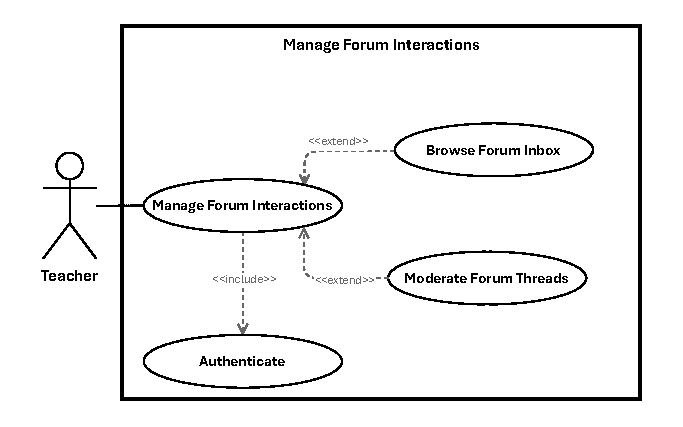
\includegraphics[width=\textwidth]{assets/chapter3/teacher-manage-forum-internaction-use-case}
    \caption{Use Case Manage Forum Interactions}
    \label{fig:teacher-manage-forum-internaction-use-case}
\end{figure}

\dotsection{\textbf{Specification of the Use Case Browse Forum Inbox}}
\begin{table}[H]
    \centering
    \caption{Use Case Specification: Browse Forum Inbox}
    \begin{tabular}{|p{3.5cm}|p{10.5cm}|}
        \hline
        \textbf{Title}          & Browse Forum Inbox \\
        \hline
        \textbf{Summary}        & Teacher opens the discussion forum inbox and filters threads by status to identify questions requiring attention \\
        \hline
        \textbf{Actor}          & Teacher \\
        \hline
        \textbf{Precondition}   & Teacher owns at least one training path with forum activity \\
        \hline
        \textbf{Post-condition} & Teacher views a filtered list of threads and may proceed to read or respond \\
        \hline
        \textbf{Basic Scenario} & \begin{minipage}[t]{\linewidth}
            \begin{enumerate}[topsep=0pt,itemsep=1pt,parsep=0pt,partopsep=0pt]
                \item Teacher navigates to the forum inbox from the teaching dashboard
                \item System displays threads from all owned training paths with reply counts and timestamps
                \item Teacher selects a filter to narrow the view:
                \begin{itemize}
                    \item \textbf{Flagged} — shows threads or replies that have been reported and require moderation
                    \item \textbf{Unanswered} — shows threads with no teacher response yet
                    \item \textbf{Recent} — shows threads sorted by most recent activity
                \end{itemize}
                \item System retrieves and displays threads matching the selected filter
                \item Teacher may select any thread to read, respond, or take a moderation action
            \end{enumerate}
        \end{minipage} \\
        \hline
        \textbf{Error Scenario} & \begin{minipage}[t]{\linewidth}
            \begin{enumerate}[topsep=0pt,itemsep=1pt,parsep=0pt,partopsep=0pt]
                \item If no threads match the active filter, system displays an empty state
                \item If filter retrieval fails, system falls back to showing all threads with an error notice
                \item If teacher has no training paths, system displays an empty state with setup instructions
            \end{enumerate}
        \end{minipage} \\
        \hline
    \end{tabular}
    \label{tab:teacher-forum-inbox}
\end{table}
\dotsection{\textbf{Specification of the Use Case Moderate Forum Threads}}
\begin{table}[H]
    \centering
    \caption{Use Case Specification: Moderate Forum Threads}
    \begin{tabular}{|p{3.5cm}|p{10.5cm}|}
        \hline
        \textbf{Title}          & Moderate Forum Threads \\
        \hline
        \textbf{Summary}        & Teacher moderates discussion threads within owned training paths by pinning, locking, resolving flags, and editing or removing inappropriate content \\
        \hline
        \textbf{Actor}          & Teacher \\
        \hline
        \textbf{Precondition}   & Teacher owns the training path containing the target thread or reply \\
        \hline
        \textbf{Post-condition} & Thread state is updated according to the moderation action performed; a log entry is created and affected engineers are notified where applicable \\
        \hline
        \textbf{Basic Scenario} & \begin{minipage}[t]{\linewidth}
            \begin{enumerate}[topsep=0pt,itemsep=1pt,parsep=0pt,partopsep=0pt]
                \item Teacher opens a thread from the forum inbox
                \item Teacher selects a moderation action:
                \begin{itemize}
                    \item \textbf{Pin / Unpin} — promotes the thread to the top of the forum listing or returns it to chronological order
                    \item \textbf{Lock / Unlock} — prevents new replies from engineers or reopens the thread for discussion
                    \item \textbf{Resolve Flag} — teacher reviews flagged content, takes appropriate action (approve, edit, or delete), then marks the flag as resolved
                    \item \textbf{Edit / Delete post} — teacher corrects or removes inappropriate content and system logs the action with timestamp and reason
                \end{itemize}
                \item System validates ownership and applies the requested state change
                \item System confirms the action and notifies affected engineers where applicable
            \end{enumerate}
        \end{minipage} \\
        \hline
        \textbf{Error Scenario} & \begin{minipage}[t]{\linewidth}
            \begin{enumerate}[topsep=0pt,itemsep=1pt,parsep=0pt,partopsep=0pt]
                \item Unauthorized access is denied if teacher does not own the training path
                \item If the target thread or post has already been removed, system displays a notice
                \item Resolving a flag on non-flagged content surfaces an explanatory error
                \item Persistence failures preserve the previous state and surface a recoverable error
            \end{enumerate}
        \end{minipage} \\
        \hline
    \end{tabular}
    \label{tab:teacher-forum-moderation}
\end{table}
\iffalse
\dotsection{\textbf{Specification of the Use Case Open Forum Inbox}}
\begin{table}[H]
    \centering
    \caption{Use Case Specification: Open Forum Inbox}
    \begin{tabular}{|p{3.5cm}|p{10.5cm}|}
        \hline
        \textbf{Title}          & Open Forum Inbox                                                                 \\
        \hline
        \textbf{Summary}        & Teacher opens discussion forum inbox to view and manage engineer questions      \\
        \hline
        \textbf{Actor}          & Teacher                                                                      \\
        \hline
        \textbf{Precondition}   & Teacher owns at least one training path with forum activity                   \\
        \hline
        \textbf{Post-condition} & Teacher views forum threads organized by priority and status                 \\
        \hline
        \textbf{Basic Scenario} & \begin{minipage}[t]{\linewidth}
                                      \begin{enumerate}[topsep=0pt,itemsep=1pt,parsep=0pt,partopsep=0pt]
                                          \item Teacher navigates to forum inbox from teaching dashboard
                                          \item System displays threads from teacher's training paths
                                          \item System organizes threads by filter (flagged, unanswered, recent)
                                          \item Teacher views thread previews with reply counts
                                          \item Teacher may select threads to read and respond
                                      \end{enumerate}
                                  \end{minipage} \\
        \hline
        \textbf{Error Scenario} & \begin{minipage}[t]{\linewidth}
                                      \begin{enumerate}[topsep=0pt,itemsep=1pt,parsep=0pt,partopsep=0pt]
                                          \item If teacher has no training paths, system displays empty state
                                          \item If no forum activity exists, system displays no threads message
                                      \end{enumerate}
                                  \end{minipage} \\
        \hline
    \end{tabular}
    \label{tab:teacher-forum-inbox}
\end{table}
\dotsection{\textbf{Specification of the Use Case Filter Flagged Threads}}
\begin{table}[H]
    \centering
    \caption{Use Case Specification: Filter Flagged Threads}
    \begin{tabular}{|p{3.5cm}|p{10.5cm}|}
        \hline
        \textbf{Title}          & Filter Flagged Threads                                                                 \\
        \hline
        \textbf{Summary}        & Teacher filters forum inbox to show only flagged threads requiring moderation \\
        \hline
        \textbf{Actor}          & Teacher                                                                      \\
        \hline
        \textbf{Precondition}   & Teacher owns training paths with forum activity and some threads are flagged \\
        \hline
        \textbf{Post-condition} & Teacher views list of flagged threads requiring attention                      \\
        \hline
        \textbf{Basic Scenario} & \begin{minipage}[t]{\linewidth}
                                      \begin{enumerate}[topsep=0pt,itemsep=1pt,parsep=0pt,partopsep=0pt]
                                          \item Teacher opens forum inbox
                                          \item Teacher selects "Flagged" filter option
                                          \item System retrieves threads with flag status
                                          \item System displays flagged threads with flag details
                                          \item Teacher may review and resolve flags
                                          \item Teacher may take moderation actions
                                      \end{enumerate}
                                  \end{minipage} \\
        \hline
        \textbf{Error Scenario} & \begin{minipage}[t]{\linewidth}
                                      \begin{enumerate}[topsep=0pt,itemsep=1pt,parsep=0pt,partopsep=0pt]
                                          \item If no flagged threads exist, system displays empty state
                                          \item If filter fails, system displays error and shows all threads
                                      \end{enumerate}
                                  \end{minipage} \\
        \hline
    \end{tabular}
    \label{tab:teacher-filter-flagged}
\end{table}
\dotsection{\textbf{Specification of the Use Case Filter Unanswered Threads}}
\begin{table}[H]
    \centering
    \caption{Use Case Specification: Filter Unanswered Threads}
    \begin{tabular}{|p{3.5cm}|p{10.5cm}|}
        \hline
        \textbf{Title}          & Filter Unanswered Threads                                                                 \\
        \hline
        \textbf{Summary}        & Teacher filters forum inbox to show only threads without teacher responses    \\
        \hline
        \textbf{Actor}          & Teacher                                                                      \\
        \hline
        \textbf{Precondition}   & Teacher owns training paths with forum activity and some threads lack answers \\
        \hline
        \textbf{Post-condition} & Teacher views list of unanswered threads requiring response                  \\
        \hline
        \textbf{Basic Scenario} & \begin{minipage}[t]{\linewidth}
                                      \begin{enumerate}[topsep=0pt,itemsep=1pt,parsep=0pt,partopsep=0pt]
                                          \item Teacher opens forum inbox
                                          \item Teacher selects "Unanswered" filter option
                                          \item System retrieves threads without teacher responses
                                          \item System displays unanswered threads with question details
                                          \item Teacher may read threads and provide answers
                                          \item Teacher may mark replies as answers
                                      \end{enumerate}
                                  \end{minipage} \\
        \hline
        \textbf{Error Scenario} & \begin{minipage}[t]{\linewidth}
                                      \begin{enumerate}[topsep=0pt,itemsep=1pt,parsep=0pt,partopsep=0pt]
                                          \item If no unanswered threads exist, system displays empty state
                                          \item If filter fails, system displays error and shows all threads
                                      \end{enumerate}
                                  \end{minipage} \\
        \hline
    \end{tabular}
    \label{tab:teacher-filter-unanswered}
\end{table}
\dotsection{\textbf{Specification of the Use Case Filter Recent Threads}}
\begin{table}[H]
    \centering
    \caption{Use Case Specification: Filter Recent Threads}
    \begin{tabular}{|p{3.5cm}|p{10.5cm}|}
        \hline
        \textbf{Title}          & Filter Recent Threads                                                                 \\
        \hline
        \textbf{Summary}        & Teacher filters forum inbox to show only the most recent threads by date      \\
        \hline
        \textbf{Actor}          & Teacher                                                                      \\
        \hline
        \textbf{Precondition}   & Teacher owns training paths with forum activity                              \\
        \hline
        \textbf{Post-condition} & Teacher views list of recent threads sorted by creation date                  \\
        \hline
        \textbf{Basic Scenario} & \begin{minipage}[t]{\linewidth}
                                      \begin{enumerate}[topsep=0pt,itemsep=1pt,parsep=0pt,partopsep=0pt]
                                          \item Teacher opens forum inbox
                                          \item Teacher selects "Recent" filter option
                                          \item System retrieves threads sorted by most recent activity
                                          \item System displays recent threads with timestamps
                                          \item Teacher may view and respond to recent discussions
                                      \end{enumerate}
                                  \end{minipage} \\
        \hline
        \textbf{Error Scenario} & \begin{minipage}[t]{\linewidth}
                                      \begin{enumerate}[topsep=0pt,itemsep=1pt,parsep=0pt,partopsep=0pt]
                                          \item If no recent threads exist, system displays empty state
                                          \item If filter fails, system displays error and shows all threads
                                      \end{enumerate}
                                  \end{minipage} \\
        \hline
    \end{tabular}
    \label{tab:teacher-filter-recent}
\end{table}
\dotsection{\textbf{Specification of the Use Case Pin / Unpin Thread}}
\begin{table}[H]
    \centering
    \caption{Use Case Specification: Pin / Unpin Thread}
    \begin{tabular}{|p{3.5cm}|p{10.5cm}|}
        \hline
        \textbf{Title}          & Pin / Unpin Thread                                                                 \\
        \hline
        \textbf{Summary}        & Teacher pins important threads to top of forum or unpins them                \\
        \hline
        \textbf{Actor}          & Teacher                                                                      \\
        \hline
        \textbf{Precondition}   & Teacher owns the training path containing the forum thread                   \\
        \hline
        \textbf{Post-condition} & Thread pin status is updated and thread position changes accordingly         \\
        \hline
        \textbf{Basic Scenario} & \begin{minipage}[t]{\linewidth}
                                      \begin{enumerate}[topsep=0pt,itemsep=1pt,parsep=0pt,partopsep=0pt]
                                          \item Teacher opens forum thread
                                          \item Teacher clicks "Pin" or "Unpin" option
                                          \item System updates thread pin status
                                          \item System confirms status change
                                          \item Pinned threads appear at top of forum listings
                                          \item Unpinned threads return to normal chronological order
                                      \end{enumerate}
                                  \end{minipage} \\
        \hline
        \textbf{Error Scenario} & \begin{minipage}[t]{\linewidth}
                                      \begin{enumerate}[topsep=0pt,itemsep=1pt,parsep=0pt,partopsep=0pt]
                                          \item If teacher does not own training path, system denies access
                                          \item If thread not found, system displays error
                                          \item If action fails, system displays error and preserves current state
                                      \end{enumerate}
                                  \end{minipage} \\
        \hline
    \end{tabular}
    \label{tab:teacher-pin-thread}
\end{table}
\dotsection{\textbf{Specification of the Use Case Lock / Unlock Thread}}
\begin{table}[H]
    \centering
    \caption{Use Case Specification: Lock / Unlock Thread}
    \begin{tabular}{|p{3.5cm}|p{10.5cm}|}
        \hline
        \textbf{Title}          & Lock / Unlock Thread                                                                 \\
        \hline
        \textbf{Summary}        & Teacher locks threads to prevent new replies or unlocks them to allow discussion \\
        \hline
        \textbf{Actor}          & Teacher                                                                      \\
        \hline
        \textbf{Precondition}   & Teacher owns the training path containing the forum thread                   \\
        \hline
        \textbf{Post-condition} & Thread lock status is updated and reply permissions change accordingly         \\
        \hline
        \textbf{Basic Scenario} & \begin{minipage}[t]{\linewidth}
                                      \begin{enumerate}[topsep=0pt,itemsep=1pt,parsep=0pt,partopsep=0pt]
                                          \item Teacher opens forum thread
                                          \item Teacher clicks "Lock" or "Unlock" option
                                          \item System updates thread lock status
                                          \item System confirms status change
                                          \item Locked threads prevent new replies from engineers
                                          \item Unlocked threads allow normal discussion
                                      \end{enumerate}
                                  \end{minipage} \\
        \hline
        \textbf{Error Scenario} & \begin{minipage}[t]{\linewidth}
                                      \begin{enumerate}[topsep=0pt,itemsep=1pt,parsep=0pt,partopsep=0pt]
                                          \item If teacher does not own training path, system denies access
                                          \item If thread not found, system displays error
                                          \item If action fails, system displays error and preserves current state
                                      \end{enumerate}
                                  \end{minipage} \\
        \hline
    \end{tabular}
    \label{tab:teacher-lock-thread}
\end{table}
\dotsection{\textbf{Specification of the Use Case Resolve Flag}}
\begin{table}[H]
    \centering
    \caption{Use Case Specification: Resolve Flag}
    \begin{tabular}{|p{3.5cm}|p{10.5cm}|}
        \hline
        \textbf{Title}          & Resolve Flag                                                                 \\
        \hline
        \textbf{Summary}        & Teacher resolves flagged content after review and removes flag status        \\
        \hline
        \textbf{Actor}          & Teacher                                                                      \\
        \hline
        \textbf{Precondition}   & Teacher owns the training path and thread or reply is flagged                \\
        \hline
        \textbf{Post-condition} & Flag status is removed and content is marked as reviewed                       \\
        \hline
        \textbf{Basic Scenario} & \begin{minipage}[t]{\linewidth}
                                      \begin{enumerate}[topsep=0pt,itemsep=1pt,parsep=0pt,partopsep=0pt]
                                          \item Teacher opens flagged thread or reply
                                          \item Teacher reviews the flagged content
                                          \item Teacher determines appropriate action (edit, delete, or approve)
                                          \item Teacher takes moderation action
                                          \item Teacher clicks "Resolve Flag" option
                                          \item System removes flag status
                                          \item System confirms resolution
                                      \end{enumerate}
                                  \end{minipage} \\
        \hline
        \textbf{Error Scenario} & \begin{minipage}[t]{\linewidth}
                                      \begin{enumerate}[topsep=0pt,itemsep=1pt,parsep=0pt,partopsep=0pt]
                                          \item If teacher does not own training path, system denies access
                                          \item If content not flagged, system displays error
                                          \item If resolution fails, system displays error
                                      \end{enumerate}
                                  \end{minipage} \\
        \hline
    \end{tabular}
    \label{tab:teacher-resolve-flag}
\end{table}
\dotsection{\textbf{Specification of the Use Case Submit VM Assignment}}
\begin{table}[H]
    \centering
    \caption{Use Case Specification: Submit VM Assignment}
    \begin{tabular}{|p{3.5cm}|p{10.5cm}|}
        \hline
        \textbf{Title}          & Submit VM Assignment                                                        \\
        \hline
        \textbf{Summary}        & Teacher creates a VM assignment request for a training unit, specifying template, duration and justification \\
        \hline
        \textbf{Actor}          & Teacher                                                                      \\
        \hline
        \textbf{Precondition}   & Teacher is authorized to request VMs for the target training unit           \\
        \hline
        \textbf{Post-condition} & A new TrainingUnitVMAssignment record is created with status "pending" and notifications dispatched as configured \\
        \hline
        \textbf{Basic Scenario} & \begin{minipage}[t]{\linewidth}
                                      \begin{enumerate}[topsep=0pt,itemsep=1pt,parsep=0pt,partopsep=0pt]
                                          \item Teacher opens the "Submit VM Assignment" form for a training unit
                                          \item Teacher selects VM template, duration and provides justification
                                          \item System validates ownership and fields, then calls service to create assignment
                                          \item System returns confirmation and lists the created assignment with status
                                      \end{enumerate}
                                  \end{minipage} \\
        \hline
        \textbf{Error Scenario} & \begin{minipage}[t]{\linewidth}
                                      \begin{enumerate}[topsep=0pt,itemsep=1pt,parsep=0pt,partopsep=0pt]
                                          \item If validation fails, display field errors and preserve input
                                          \item If quota or node availability prevents assignment, show an explanatory error
                                      \end{enumerate}
                                  \end{minipage} \\
        \hline
    \end{tabular}
    \label{tab:teacher-submit-vm-assignment}
\end{table}
\fi

\subsubsubsection[Manage VM Assignments]{Refinement of the Use Case Manage VM Assignments} Figure
\ref{fig:teacher-manage-vm-assignments-use-case} presents the refinement of the
Use Case Manage VM Assignments for the Teacher actor. This use case includes
the following sub-use cases:
\dotsection{\textbf{Specification of the Use Case Submit VM Assignment}}
\begin{table}[H]
    \centering
    \caption{Use Case Specification: Submit VM Assignment}
    \begin{tabular}{|p{3.5cm}|p{10.5cm}|}
        \hline
        \textbf{Title}          & Submit VM Assignment \\
        \hline
        \textbf{Summary}        & Teacher creates a VM assignment request for a training unit, specifying template, duration, and justification \\
        \hline
        \textbf{Actor}          & Teacher \\
        \hline
        \textbf{Precondition}   & Teacher is authorized to request VMs for the target training unit \\
        \hline
        \textbf{Post-condition} & A new VM assignment record is created with pending status and notifications are dispatched as configured \\
        \hline
        \textbf{Basic Scenario} & \begin{minipage}[t]{\linewidth}
            \begin{enumerate}[topsep=0pt,itemsep=1pt,parsep=0pt,partopsep=0pt]
                \item Teacher opens the VM assignment form for a training unit
                \item Teacher selects a VM template and duration, and provides a justification
                \item System validates ownership and field values, then creates the assignment record
                \item System confirms submission and displays the new assignment with its pending status
            \end{enumerate}
        \end{minipage} \\
        \hline
        \textbf{Error Scenario} & \begin{minipage}[t]{\linewidth}
            \begin{enumerate}[topsep=0pt,itemsep=1pt,parsep=0pt,partopsep=0pt]
                \item Validation failures surface field-level errors and preserve input
                \item If quota or node availability prevents assignment, system displays an explanatory error
            \end{enumerate}
        \end{minipage} \\
        \hline
    \end{tabular}
    \label{tab:teacher-submit-vm-assignment}
\end{table}
\dotsection{\textbf{Specification of the Use Case Manage Assignments}}
\begin{table}[H]
    \centering
    \caption{Use Case Specification: Manage VM Assignments}
    \begin{tabular}{|p{3.5cm}|p{10.5cm}|}
        \hline
        \textbf{Title}          & Manage VM Assignments \\
        \hline
        \textbf{Summary}        & Teacher views and cancels VM assignment requests associated with their training paths \\
        \hline
        \textbf{Actor}          & Teacher \\
        \hline
        \textbf{Precondition}   & Teacher is authenticated and associated with at least one training path \\
        \hline
        \textbf{Post-condition} & Teacher views current assignments or a selected assignment is cancelled and any scheduled provisioning is aborted \\
        \hline
        \textbf{Basic Scenario} & \begin{minipage}[t]{\linewidth}
            \begin{enumerate}[topsep=0pt,itemsep=1pt,parsep=0pt,partopsep=0pt]
                \item Teacher opens the VM assignments view
                \item System displays assignments grouped by training path with status, template, and timestamps
                \item Teacher may filter or sort the list, or open an assignment for details
                \item To cancel, teacher selects an assignment and confirms the delete action
                \item System verifies the assignment is in a cancellable state, removes or marks it cancelled, and updates the list
            \end{enumerate}
        \end{minipage} \\
        \hline
        \textbf{Error Scenario} & \begin{minipage}[t]{\linewidth}
            \begin{enumerate}[topsep=0pt,itemsep=1pt,parsep=0pt,partopsep=0pt]
                \item If no assignments exist, system displays an empty state with setup instructions
                \item If the assignment is already provisioned or in a non-cancellable state, system displays an explanatory error
                \item Persistence failures preserve current state and surface a recoverable error
            \end{enumerate}
        \end{minipage} \\
        \hline
    \end{tabular}
    \label{tab:teacher-manage-vm-assignments}
\end{table}

\iffalse
\begin{figure}[H]
    \centering
    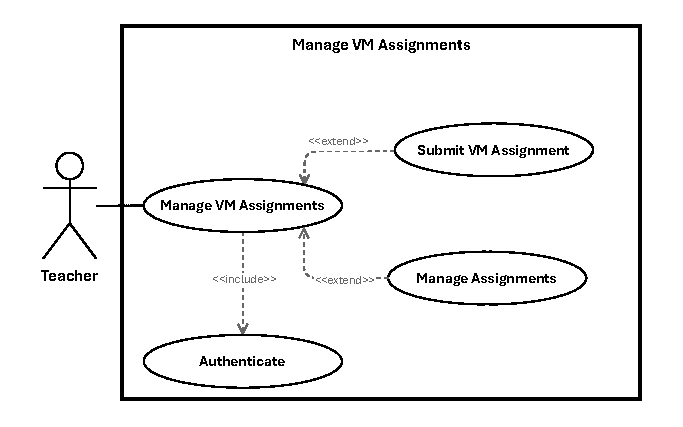
\includegraphics[width=\textwidth]{assets/chapter3/teacher-manage-vm-assignments-use-case}
    \caption{Use Case Manage VM Assignments}
    \label{fig:teacher-manage-vm-assignments-use-case}
\end{figure}
\dotsection{\textbf{Specification of the Use Case View My VM Assignments}}
\begin{table}[H]
    \centering
    \caption{Use Case Specification: View My VM Assignments}
    \begin{tabular}{|p{3.5cm}|p{10.5cm}|}
        \hline
        \textbf{Title}          & View My VM Assignments                                                      \\
        \hline
        \textbf{Summary}        & Teacher views VM assignment requests they have created or that belong to their training paths (see repository behaviour) \\
        \hline
        \textbf{Actor}          & Teacher                                                                      \\
        \hline
        \textbf{Precondition}   & Teacher is authenticated and associated with at least one training path      \\
        \hline
        \textbf{Post-condition} & Teacher sees a list of assignments with status, assigned unit, VM template and timestamps \\
        \hline
        \textbf{Basic Scenario} & \begin{minipage}[t]{\linewidth}
                                      \begin{enumerate}[topsep=0pt,itemsep=1pt,parsep=0pt,partopsep=0pt]
                                          \item Teacher opens "My VM Assignments" view
                                          \item System queries TrainingUnitVMAssignmentRepository::findByTeacher and returns assignments
                                          \item System displays assignments grouped by training path/module with status indicators
                                          \item Teacher may filter, sort, or open an assignment for details
                                      \end{enumerate}
                                  \end{minipage} \\
        \hline
        \textbf{Error Scenario} & \begin{minipage}[t]{\linewidth}
                                      \begin{enumerate}[topsep=0pt,itemsep=1pt,parsep=0pt,partopsep=0pt]
                                          \item If repository call fails, display an error and suggest retrying
                                          \item If there are no assignments, show an empty state with instructions
                                      \end{enumerate}
                                  \end{minipage} \\
        \hline
    \end{tabular}
    \label{tab:teacher-view-my-vm-assignments}
\end{table}
\dotsection{\textbf{Specification of the Use Case Delete VM Assignment}}
\begin{table}[H]
    \centering
    \caption{Use Case Specification: Delete VM Assignment}
    \begin{tabular}{|p{3.5cm}|p{10.5cm}|}
        \hline
        \textbf{Title}          & Delete VM Assignment                                                        \\
        \hline
        \textbf{Summary}        & Teacher deletes or cancels a previously submitted VM assignment when it is no longer required \\
        \hline
        \textbf{Actor}          & Teacher                                                                      \\
        \hline
        \textbf{Precondition}   & Assignment exists and is in a deletable state (e.g. pending or approved but not yet provisioned) \\
        \hline
        \textbf{Post-condition} & Assignment record is removed or marked cancelled; any scheduled provisioning is aborted and notifications sent as appropriate \\
        \hline
        \textbf{Basic Scenario} & \begin{minipage}[t]{\linewidth}
                                      \begin{enumerate}[topsep=0pt,itemsep=1pt,parsep=0pt,partopsep=0pt]
                                          \item Teacher selects an assignment and chooses "Delete/Cancel"
                                          \item System confirms the action with the user
                                          \item System verifies deletable state and calls repository/service to cancel the assignment
                                          \item System returns success and updates the assignment list
                                      \end{enumerate}
                                  \end{minipage} \\
        \hline
        \textbf{Error Scenario} & \begin{minipage}[t]{\linewidth}
                                      \begin{enumerate}[topsep=0pt,itemsep=1pt,parsep=0pt,partopsep=0pt]
                                          \item If assignment is already provisioned or in a non-deletable state, show an explanatory error
                                          \item If the delete operation fails, display an error and preserve current state
                                      \end{enumerate}
                                  \end{minipage} \\
        \hline
    \end{tabular}
    \label{tab:teacher-delete-vm-assignment}
\end{table}
\fi

\dotsection{\textbf{Specification of the Use Case Manage Earnings \& Payouts}}
\begin{table}[H]
    \centering
    \caption{Use Case Specification: Manage Earnings \& Payouts}
    \begin{tabular}{|p{3.5cm}|p{10.5cm}|}
        \hline
        \textbf{Title}          & Manage Earnings \& Payouts \\
        \hline
        \textbf{Summary}        & Teacher views their earnings summary, requests a payout of available balance, and exports transaction history as a CSV report \\
        \hline
        \textbf{Actor}          & Teacher \\
        \hline
        \textbf{Precondition}   & Teacher is authenticated and has at least one training path with paid enrollments \\
        \hline
        \textbf{Post-condition} & Teacher has viewed financial data, submitted a payout request, or downloaded an earnings report according to the action performed \\
        \hline
        \textbf{Basic Scenario} & \begin{minipage}[t]{\linewidth}
            \begin{enumerate}[topsep=0pt,itemsep=1pt,parsep=0pt,partopsep=0pt]
                \item Teacher navigates to the earnings section
                \item System displays total earnings, available balance, pending payouts, and a revenue breakdown by training path; teacher may filter by date range
                \item For \textbf{Request Payout}: teacher enters the desired amount and selects a payment method; system validates the amount against the available balance and minimum threshold, creates a pending payout request, and confirms submission
                \item For \textbf{Export Report}: teacher specifies a date range and clicks export; system generates a CSV file of transaction details and initiates the download
            \end{enumerate}
        \end{minipage} \\
        \hline
        \textbf{Error Scenario} & \begin{minipage}[t]{\linewidth}
            \begin{enumerate}[topsep=0pt,itemsep=1pt,parsep=0pt,partopsep=0pt]
                \item If no earnings data exists, system displays an empty state
                \item Payout amount exceeding available balance or falling below the minimum threshold surfaces a specific validation error
                \item Invalid payment method prevents payout submission
                \item An invalid or empty date range prevents CSV export
                \item Service or export failures surface a recoverable error with a retry option
            \end{enumerate}
        \end{minipage} \\
        \hline
    \end{tabular}
    \label{tab:teacher-earnings}
\end{table}
\iffalse
\subsubsubsection[Manage Earnings \& Payouts]{Refinement of the Use Case Manage Earnings \& Payouts} Figure
\ref{fig:teacher-manage-earnings-and-payouts-use-case} presents the refinement of the
Use Case Manage Earnings \& Payouts for the Teacher actor. This use case includes
the following sub-use cases:
\begin{figure}[H]
    \centering
    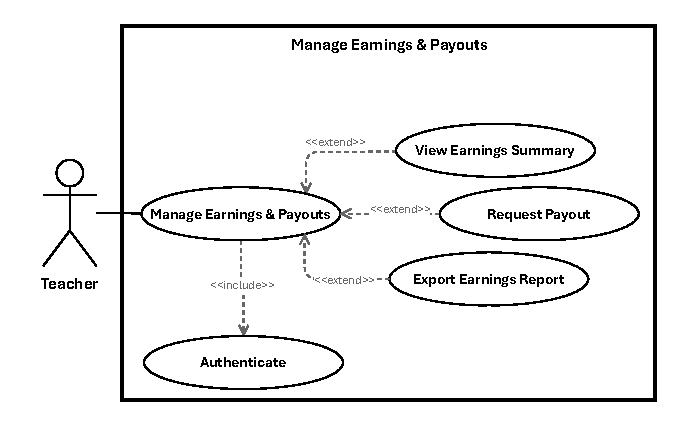
\includegraphics[width=\textwidth]{assets/chapter3/teacher-manage-earnings-and-payouts-use-case}
    \caption{Use Case Manage Earnings \& Payouts}
    \label{fig:teacher-manage-earnings-and-payouts-use-case}
\end{figure}
\dotsection{\textbf{Specification of the Use Case View Earnings Summary}}
\begin{table}[H]
    \centering
    \caption{Use Case Specification: View Earnings Summary}
    \begin{tabular}{|p{3.5cm}|p{10.5cm}|}
        \hline
        \textbf{Title}          & View Earnings Summary                                                                 \\
        \hline
        \textbf{Summary}        & Teacher views earnings summary including total revenue, available balance, and pending payouts \\
        \hline
        \textbf{Actor}          & Teacher                                                                      \\
        \hline
        \textbf{Precondition}   & Teacher is authenticated and has training paths with paid enrollments         \\
        \hline
        \textbf{Post-condition} & Teacher views comprehensive earnings summary with financial breakdown          \\
        \hline
        \textbf{Basic Scenario} & \begin{minipage}[t]{\linewidth}
                                      \begin{enumerate}[topsep=0pt,itemsep=1pt,parsep=0pt,partopsep=0pt]
                                          \item Teacher navigates to earnings section
                                          \item System retrieves earnings data
                                          \item System displays total earnings, available balance, pending payouts
                                          \item System shows revenue breakdown by training path
                                          \item System displays transaction history
                                          \item Teacher may filter by date range
                                      \end{enumerate}
                                  \end{minipage} \\
        \hline
        \textbf{Error Scenario} & \begin{minipage}[t]{\linewidth}
                                      \begin{enumerate}[topsep=0pt,itemsep=1pt,parsep=0pt,partopsep=0pt]
                                          \item If no earnings data exists, system displays empty state
                                          \item If earnings service unavailable, system shows error
                                      \end{enumerate}
                                  \end{minipage} \\
        \hline
    \end{tabular}
    \label{tab:teacher-earnings-summary}
\end{table}
\dotsection{\textbf{Specification of the Use Case Request Payout}}
\begin{table}[H]
    \centering
    \caption{Use Case Specification: Request Payout}
    \begin{tabular}{|p{3.5cm}|p{10.5cm}|}
        \hline
        \textbf{Title}          & Request Payout                                                                 \\
        \hline
        \textbf{Summary}        & Teacher requests payout of available earnings to their designated payment method \\
        \hline
        \textbf{Actor}          & Teacher                                                                      \\
        \hline
        \textbf{Precondition}   & Teacher has available balance above minimum payout threshold                   \\
        \hline
        \textbf{Post-condition} & Payout request is created and submitted for administrator processing          \\
        \hline
        \textbf{Basic Scenario} & \begin{minipage}[t]{\linewidth}
                                      \begin{enumerate}[topsep=0pt,itemsep=1pt,parsep=0pt,partopsep=0pt]
                                          \item Teacher navigates to earnings section
                                          \item Teacher views available balance
                                          \item Teacher clicks "Request Payout" button
                                          \item System displays payout request form
                                          \item Teacher enters payout amount and selects payment method
                                          \item Teacher submits payout request
                                          \item System validates amount against available balance
                                          \item System creates payout request with pending status
                                          \item System confirms submission
                                      \end{enumerate}
                                  \end{minipage} \\
        \hline
        \textbf{Error Scenario} & \begin{minipage}[t]{\linewidth}
                                      \begin{enumerate}[topsep=0pt,itemsep=1pt,parsep=0pt,partopsep=0pt]
                                          \item If amount exceeds available balance, system displays error
                                          \item If amount below minimum threshold, system displays minimum required
                                          \item If payout method invalid, system displays error
                                      \end{enumerate}
                                  \end{minipage} \\
        \hline
    \end{tabular}
    \label{tab:teacher-request-payout}
\end{table}
\dotsection{\textbf{Specification of the Use Case Export Earnings Report}}
\begin{table}[H]
    \centering
    \caption{Use Case Specification: Export Earnings Report}
    \begin{tabular}{|p{3.5cm}|p{10.5cm}|}
        \hline
        \textbf{Title}          & Export Earnings Report                                                                 \\
        \hline
        \textbf{Summary}        & Teacher exports earnings data to CSV file for accounting and record keeping   \\
        \hline
        \textbf{Actor}          & Teacher                                                                      \\
        \hline
        \textbf{Precondition}   & Teacher is authenticated and has earnings data to export                    \\
        \hline
        \textbf{Post-condition} & CSV file containing earnings data is downloaded to teacher's device         \\
        \hline
        \textbf{Basic Scenario} & \begin{minipage}[t]{\linewidth}
                                      \begin{enumerate}[topsep=0pt,itemsep=1pt,parsep=0pt,partopsep=0pt]
                                          \item Teacher navigates to earnings section
                                          \item Teacher specifies date range for export
                                          \item Teacher clicks "Export CSV" button
                                          \item System retrieves earnings data for specified period
                                          \item System generates CSV file with transaction details
                                          \item System initiates file download
                                          \item Teacher saves CSV file to device
                                      \end{enumerate}
                                  \end{minipage} \\
        \hline
        \textbf{Error Scenario} & \begin{minipage}[t]{\linewidth}
                                      \begin{enumerate}[topsep=0pt,itemsep=1pt,parsep=0pt,partopsep=0pt]
                                          \item If no earnings data for period, system displays empty CSV
                                          \item If export fails, system displays error and retry option
                                          \item If date range invalid, system displays validation error
                                      \end{enumerate}
                                  \end{minipage} \\
        \hline
    \end{tabular}
    \label{tab:teacher-export-earnings}
\end{table}
\fi
